% Options for packages loaded elsewhere
\PassOptionsToPackage{unicode}{hyperref}
\PassOptionsToPackage{hyphens}{url}
%
\documentclass[
  ignorenonframetext,
]{beamer}
\usepackage{pgfpages}
\setbeamertemplate{caption}[numbered]
\setbeamertemplate{caption label separator}{: }
\setbeamercolor{caption name}{fg=normal text.fg}
\beamertemplatenavigationsymbolsempty
% Prevent slide breaks in the middle of a paragraph
\widowpenalties 1 10000
\raggedbottom
\setbeamertemplate{part page}{
  \centering
  \begin{beamercolorbox}[sep=16pt,center]{part title}
    \usebeamerfont{part title}\insertpart\par
  \end{beamercolorbox}
}
\setbeamertemplate{section page}{
  \centering
  \begin{beamercolorbox}[sep=12pt,center]{part title}
    \usebeamerfont{section title}\insertsection\par
  \end{beamercolorbox}
}
\setbeamertemplate{subsection page}{
  \centering
  \begin{beamercolorbox}[sep=8pt,center]{part title}
    \usebeamerfont{subsection title}\insertsubsection\par
  \end{beamercolorbox}
}
\AtBeginPart{
  \frame{\partpage}
}
\AtBeginSection{
  \ifbibliography
  \else
    \frame{\sectionpage}
  \fi
}
\AtBeginSubsection{
  \frame{\subsectionpage}
}
\usepackage{lmodern}
\usepackage{amssymb,amsmath}
\usepackage{ifxetex,ifluatex}
\ifnum 0\ifxetex 1\fi\ifluatex 1\fi=0 % if pdftex
  \usepackage[T1]{fontenc}
  \usepackage[utf8]{inputenc}
  \usepackage{textcomp} % provide euro and other symbols
\else % if luatex or xetex
  \usepackage{unicode-math}
  \defaultfontfeatures{Scale=MatchLowercase}
  \defaultfontfeatures[\rmfamily]{Ligatures=TeX,Scale=1}
\fi
% Use upquote if available, for straight quotes in verbatim environments
\IfFileExists{upquote.sty}{\usepackage{upquote}}{}
\IfFileExists{microtype.sty}{% use microtype if available
  \usepackage[]{microtype}
  \UseMicrotypeSet[protrusion]{basicmath} % disable protrusion for tt fonts
}{}
\makeatletter
\@ifundefined{KOMAClassName}{% if non-KOMA class
  \IfFileExists{parskip.sty}{%
    \usepackage{parskip}
  }{% else
    \setlength{\parindent}{0pt}
    \setlength{\parskip}{6pt plus 2pt minus 1pt}}
}{% if KOMA class
  \KOMAoptions{parskip=half}}
\makeatother
\usepackage{xcolor}
\IfFileExists{xurl.sty}{\usepackage{xurl}}{} % add URL line breaks if available
\IfFileExists{bookmark.sty}{\usepackage{bookmark}}{\usepackage{hyperref}}
\hypersetup{
  pdftitle={An introduction to hidden markov models for time series},
  pdfauthor={Eric Ward},
  hidelinks,
  pdfcreator={LaTeX via pandoc}}
\urlstyle{same} % disable monospaced font for URLs
\newif\ifbibliography
\usepackage{color}
\usepackage{fancyvrb}
\newcommand{\VerbBar}{|}
\newcommand{\VERB}{\Verb[commandchars=\\\{\}]}
\DefineVerbatimEnvironment{Highlighting}{Verbatim}{commandchars=\\\{\}}
% Add ',fontsize=\small' for more characters per line
\usepackage{framed}
\definecolor{shadecolor}{RGB}{248,248,248}
\newenvironment{Shaded}{\begin{snugshade}}{\end{snugshade}}
\newcommand{\AlertTok}[1]{\textcolor[rgb]{0.94,0.16,0.16}{#1}}
\newcommand{\AnnotationTok}[1]{\textcolor[rgb]{0.56,0.35,0.01}{\textbf{\textit{#1}}}}
\newcommand{\AttributeTok}[1]{\textcolor[rgb]{0.77,0.63,0.00}{#1}}
\newcommand{\BaseNTok}[1]{\textcolor[rgb]{0.00,0.00,0.81}{#1}}
\newcommand{\BuiltInTok}[1]{#1}
\newcommand{\CharTok}[1]{\textcolor[rgb]{0.31,0.60,0.02}{#1}}
\newcommand{\CommentTok}[1]{\textcolor[rgb]{0.56,0.35,0.01}{\textit{#1}}}
\newcommand{\CommentVarTok}[1]{\textcolor[rgb]{0.56,0.35,0.01}{\textbf{\textit{#1}}}}
\newcommand{\ConstantTok}[1]{\textcolor[rgb]{0.00,0.00,0.00}{#1}}
\newcommand{\ControlFlowTok}[1]{\textcolor[rgb]{0.13,0.29,0.53}{\textbf{#1}}}
\newcommand{\DataTypeTok}[1]{\textcolor[rgb]{0.13,0.29,0.53}{#1}}
\newcommand{\DecValTok}[1]{\textcolor[rgb]{0.00,0.00,0.81}{#1}}
\newcommand{\DocumentationTok}[1]{\textcolor[rgb]{0.56,0.35,0.01}{\textbf{\textit{#1}}}}
\newcommand{\ErrorTok}[1]{\textcolor[rgb]{0.64,0.00,0.00}{\textbf{#1}}}
\newcommand{\ExtensionTok}[1]{#1}
\newcommand{\FloatTok}[1]{\textcolor[rgb]{0.00,0.00,0.81}{#1}}
\newcommand{\FunctionTok}[1]{\textcolor[rgb]{0.00,0.00,0.00}{#1}}
\newcommand{\ImportTok}[1]{#1}
\newcommand{\InformationTok}[1]{\textcolor[rgb]{0.56,0.35,0.01}{\textbf{\textit{#1}}}}
\newcommand{\KeywordTok}[1]{\textcolor[rgb]{0.13,0.29,0.53}{\textbf{#1}}}
\newcommand{\NormalTok}[1]{#1}
\newcommand{\OperatorTok}[1]{\textcolor[rgb]{0.81,0.36,0.00}{\textbf{#1}}}
\newcommand{\OtherTok}[1]{\textcolor[rgb]{0.56,0.35,0.01}{#1}}
\newcommand{\PreprocessorTok}[1]{\textcolor[rgb]{0.56,0.35,0.01}{\textit{#1}}}
\newcommand{\RegionMarkerTok}[1]{#1}
\newcommand{\SpecialCharTok}[1]{\textcolor[rgb]{0.00,0.00,0.00}{#1}}
\newcommand{\SpecialStringTok}[1]{\textcolor[rgb]{0.31,0.60,0.02}{#1}}
\newcommand{\StringTok}[1]{\textcolor[rgb]{0.31,0.60,0.02}{#1}}
\newcommand{\VariableTok}[1]{\textcolor[rgb]{0.00,0.00,0.00}{#1}}
\newcommand{\VerbatimStringTok}[1]{\textcolor[rgb]{0.31,0.60,0.02}{#1}}
\newcommand{\WarningTok}[1]{\textcolor[rgb]{0.56,0.35,0.01}{\textbf{\textit{#1}}}}
\usepackage{longtable,booktabs}
\usepackage{caption}
% Make caption package work with longtable
\makeatletter
\def\fnum@table{\tablename~\thetable}
\makeatother
\usepackage{graphicx,grffile}
\makeatletter
\def\maxwidth{\ifdim\Gin@nat@width>\linewidth\linewidth\else\Gin@nat@width\fi}
\def\maxheight{\ifdim\Gin@nat@height>\textheight\textheight\else\Gin@nat@height\fi}
\makeatother
% Scale images if necessary, so that they will not overflow the page
% margins by default, and it is still possible to overwrite the defaults
% using explicit options in \includegraphics[width, height, ...]{}
\setkeys{Gin}{width=\maxwidth,height=\maxheight,keepaspectratio}
% Set default figure placement to htbp
\makeatletter
\def\fps@figure{htbp}
\makeatother
\setlength{\emergencystretch}{3em} % prevent overfull lines
\providecommand{\tightlist}{%
  \setlength{\itemsep}{0pt}\setlength{\parskip}{0pt}}
\setcounter{secnumdepth}{-\maxdimen} % remove section numbering

\title{An introduction to hidden markov models for time series}
\subtitle{FISH 507 -- Applied Time Series Analysis}
\author{Eric Ward}
\date{4 Feb 2021}

\begin{document}
\frame{\titlepage}

\begin{frame}{Overview of today's material}
\protect\hypertarget{overview-of-todays-material}{}

\begin{itemize}
\item
  Gentle introduction to HMMs
\item
  Theory and notation
\item
  Examples of univariate HMMs in R
\item
  Examples of multivariate HMMs in R
\end{itemize}

\end{frame}

\begin{frame}{Overview of today's material}
\protect\hypertarget{overview-of-todays-material-1}{}

For additional background, see

\begin{itemize}
\item
  Zucchini et al.~(2008, 2016) ``Hidden Markov Models for Time Series:
  An Introduction Using R''
\item
  Jackson (2011) ``Multi-State Models for Panel Data: The msm Package
  for R''
\item
  Visser and Speekenbrink (2010) ``depmixS4: An R Package for Hidden
  Markov Models''
\item
  McClintock et al.~(2020) ``Uncovering ecological state dynamics with
  hidden Markov models''
\end{itemize}

\end{frame}

\begin{frame}{State space models}
\protect\hypertarget{state-space-models}{}

We've already discussed state space models. These models include

\begin{itemize}
\item
  a latent process model (we don't directly observe)
\item
  a data or observation model
\item
  we've generally assumed both models be normal (or multivariate normal)
\end{itemize}

\end{frame}

\begin{frame}{State space models}
\protect\hypertarget{state-space-models-1}{}

Process model: \[{ x }_{ t }={ x }_{ t-1 }+{ \varepsilon  }_{ t-1 }\]

Observation model: \[{ y }_{ t }={ x }_{ t }+{ \delta  }_{ t }\]

where
\({ \varepsilon }_{ t } \sim Normal\left( 0,{ \sigma }_{ \varepsilon } \right)\)
and
\({ \delta }_{ t } \sim Normal\left( 0,{ \sigma }_{ \delta } \right)\)

\end{frame}

\begin{frame}{State space models}
\protect\hypertarget{state-space-models-2}{}

Adding AR coefficients can make these models stationary with respect to
the mean,

\[{ x }_{ t }={ p\cdot x }_{ t-1 }+{ \varepsilon  }_{ t-1 }\]

however they may not be able to explain some datasets very well.

\begin{itemize}
\tightlist
\item
  Specifically, these models are not well designed to model regimes
\end{itemize}

\end{frame}

\begin{frame}{Regimes}
\protect\hypertarget{regimes}{}

\begin{figure}
\hypertarget{id}{%
\centering
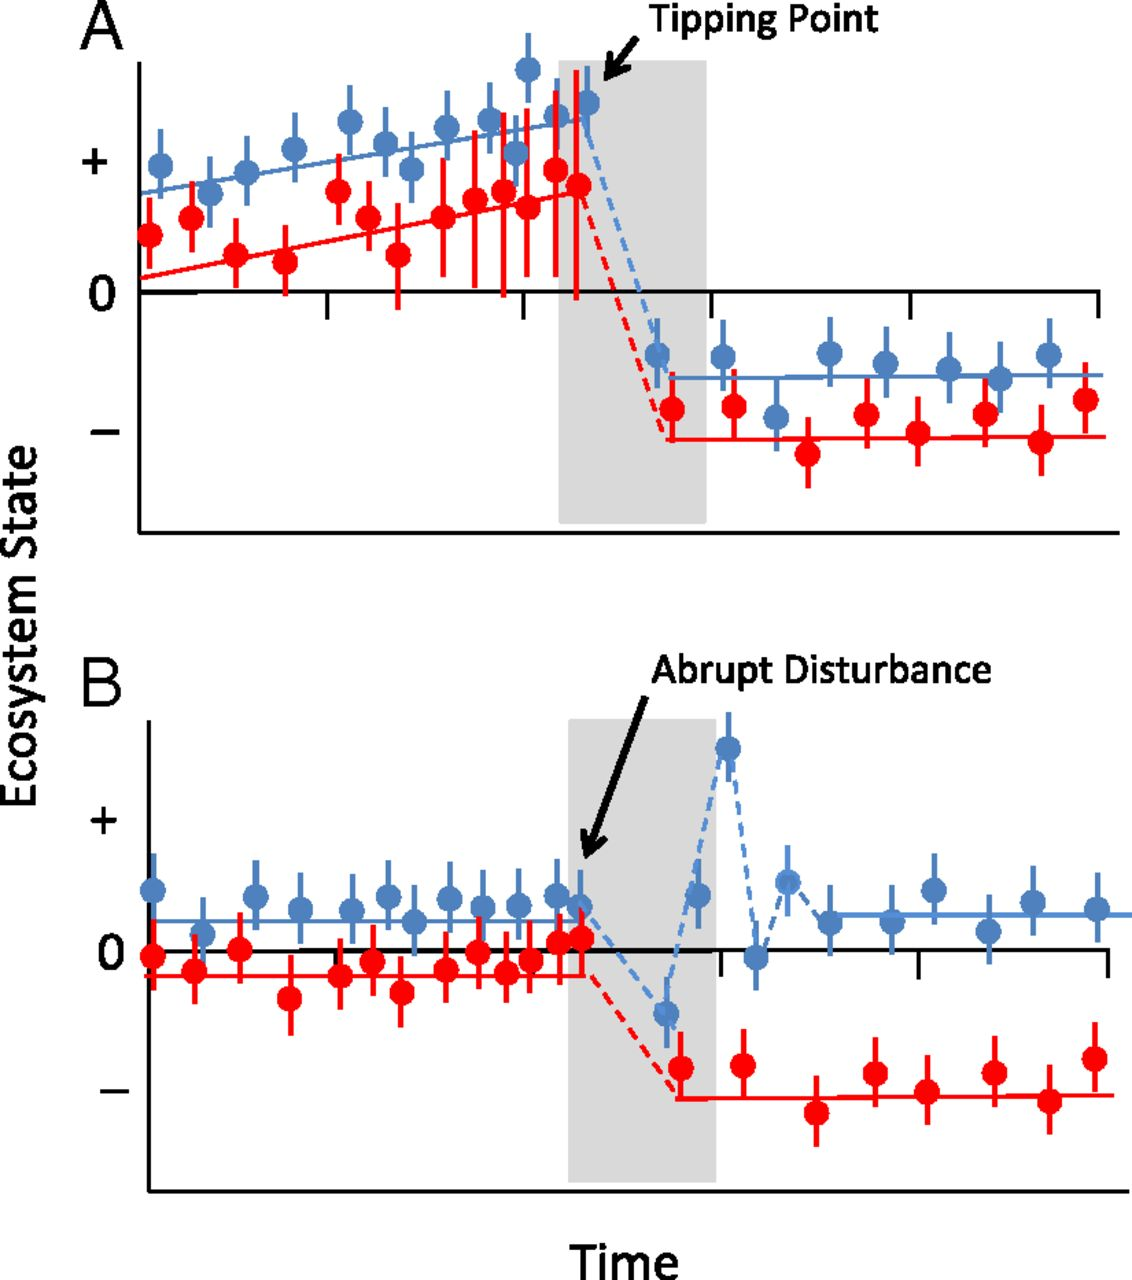
\includegraphics[width=0.5\textwidth,height=0.5\textheight]{Moore_2018.jpg}
\caption{Example from Moore (2018), ``Predicting tipping points in
complex environmental systems''}\label{id}
}
\end{figure}

\end{frame}

\begin{frame}{Regimes / behavioral states}
\protect\hypertarget{regimes-behavioral-states}{}

Many examples of time series in ecology \& fisheries may alternate
between multiple states (2+)

\begin{itemize}
\item
  Vert-pre et al.~(2013)
  \url{https://www.ncbi.nlm.nih.gov/pmc/articles/PMC3562848/}
\item
  Francis et al.~(2012)
  \url{https://onlinelibrary.wiley.com/doi/full/10.1111/j.1365-2486.2012.02702.x}
\end{itemize}

\end{frame}

\begin{frame}{Additional ecological exmaples:}
\protect\hypertarget{additional-ecological-exmaples}{}

\begin{itemize}
\item
  Mark recapture models with latent states
\item
  Identifying changing behavior or habitat use:
\item
  Tennessen et al.~(2019) ``Hidden Markov models reveal temporal
  patterns and sex differences in killer whale behavior''
\item
  Leos-Barajas et al.~(2017) ``Analysis of animal accelerometer data
  using hidden Markov models''
\item
  momentuHMM: R package for analysis of telemetry data using generalized
  multivariate hidden Markov models of animal movement
\end{itemize}

\end{frame}

\begin{frame}{Regimes}
\protect\hypertarget{regimes-1}{}

Lots of non-HMM approaches for detecting regimes

\begin{itemize}
\tightlist
\item
  STARS algorithm

  \begin{itemize}
  \tightlist
  \item
    Sequential t-test approach for detecting changes in the mean
  \item
    Rodionov (2015) \url{https://www.mdpi.com/2225-1154/3/3/474}
  \end{itemize}
\item
  Brute force model selection approach

  \begin{itemize}
  \tightlist
  \item
    iterate through change points, evaluating data support for each
  \item
    how do we do change points with regression?
    \({ Y }_{ t }=B{ X }_{ t }+{ \varepsilon }_{ t }\)
  \end{itemize}
\end{itemize}

\end{frame}

\begin{frame}{Regimes: simulating data}
\protect\hypertarget{regimes-simulating-data}{}

\begin{center}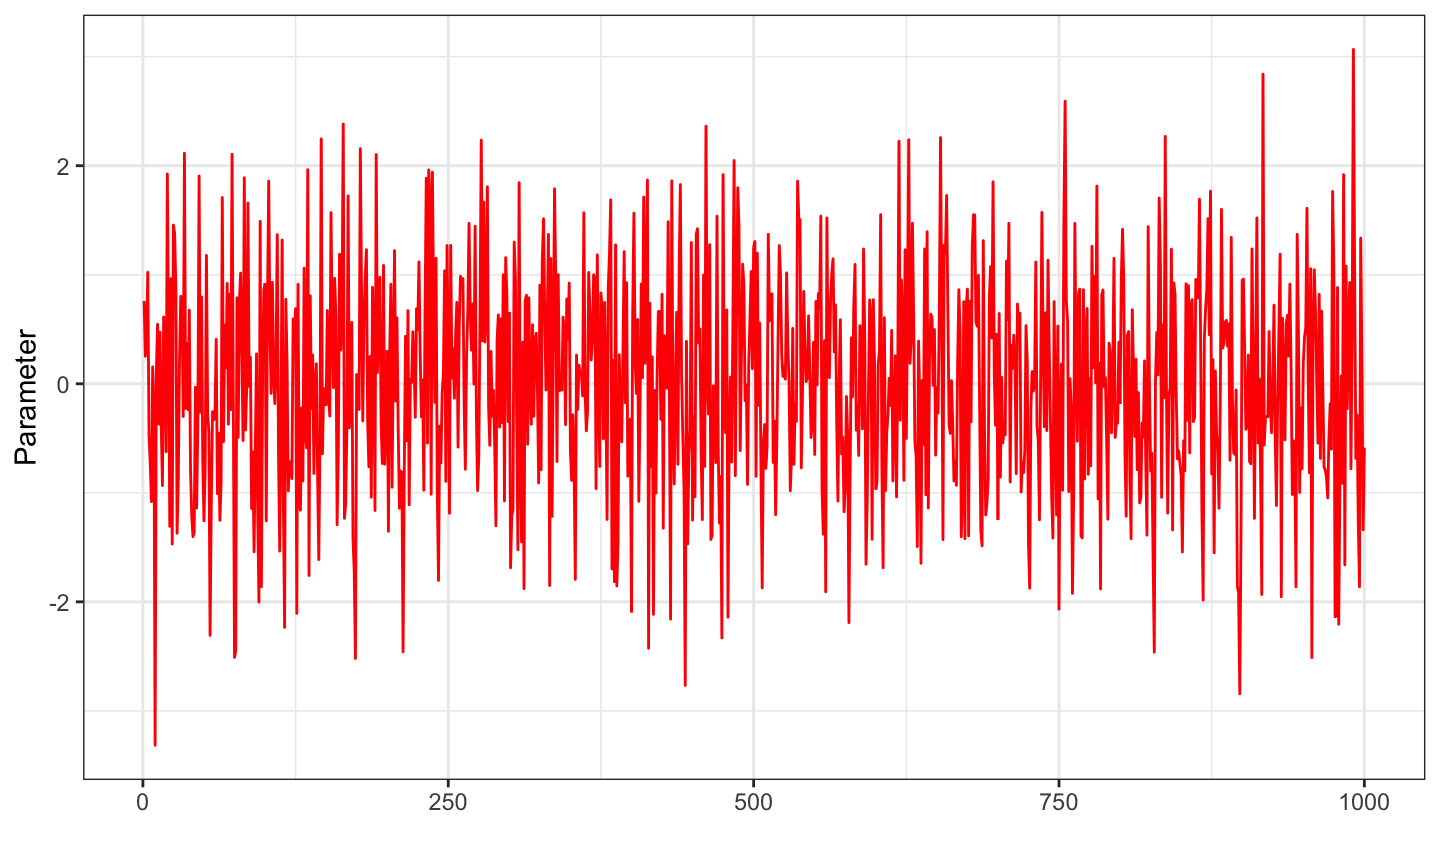
\includegraphics{lec_10_hmm_files/figure-beamer/unnamed-chunk-1-1} \end{center}

\end{frame}

\begin{frame}{Fitting these data with state space models}
\protect\hypertarget{fitting-these-data-with-state-space-models}{}

They can actually fit the data from a regime model quite well.

\begin{itemize}
\tightlist
\item
  Via MARSS()
\end{itemize}

\begin{center}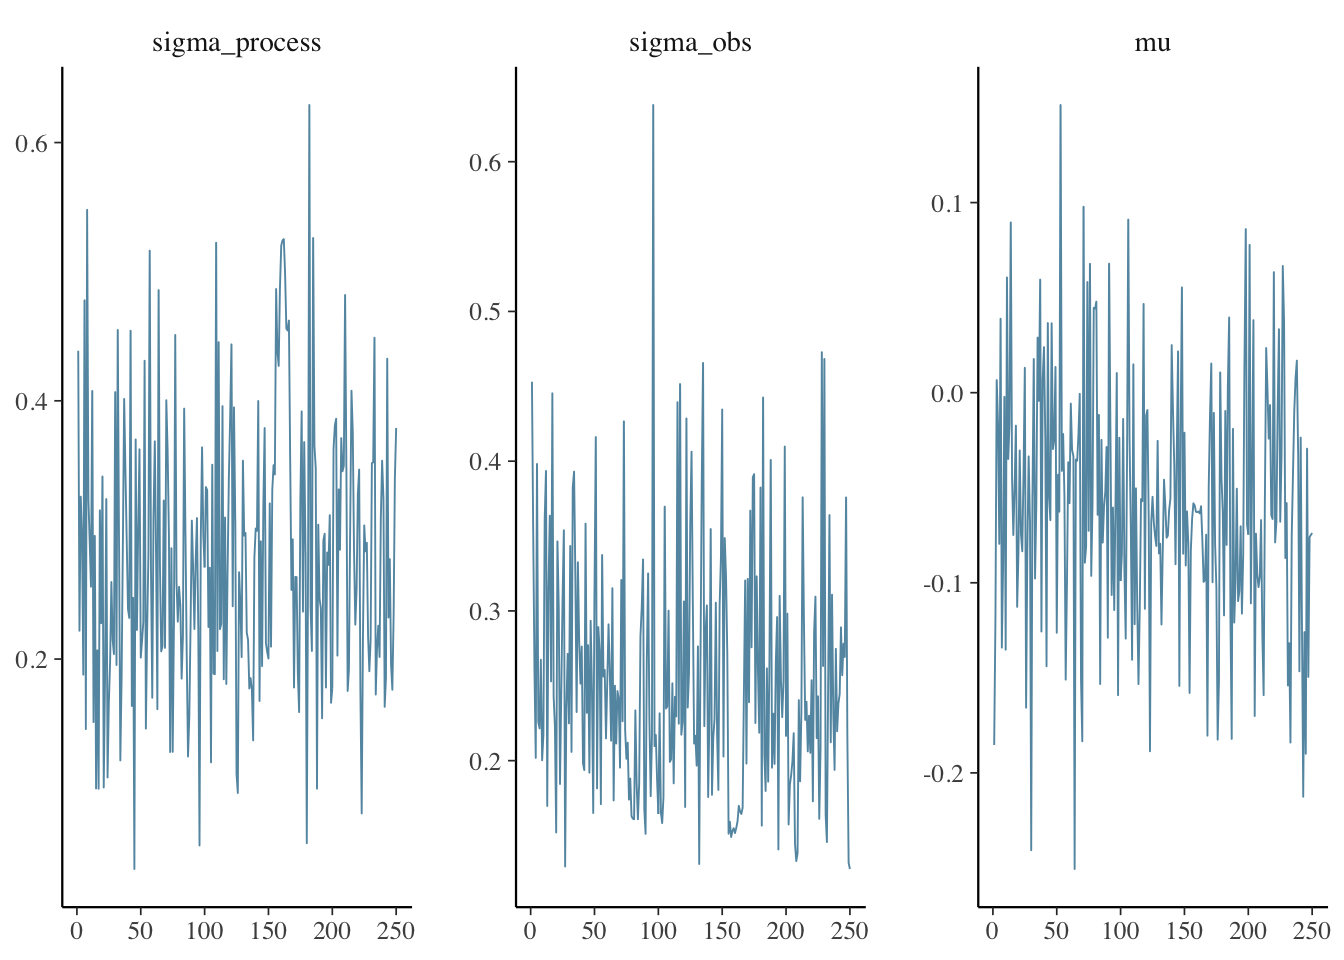
\includegraphics{lec_10_hmm_files/figure-beamer/unnamed-chunk-2-1} \end{center}

\end{frame}

\begin{frame}{Limitations of state space models with continuous states}
\protect\hypertarget{limitations-of-state-space-models-with-continuous-states}{}

What's lacking is inference about:

\begin{itemize}
\tightlist
\item
  What's the probability of transition between regimes?
\item
  How long are regimes expected to last?
\item
  What regimes might we expect in the future?
\end{itemize}

Lots of applications: speech recognition, bioinformatics, animal
movement, environmental data (rain), finance

\end{frame}

\begin{frame}{HMM: theory}
\protect\hypertarget{hmm-theory}{}

Markov Process

\begin{itemize}
\tightlist
\item
  time may be discrete or continuous (we'll focus on discrete)
\item
  Markov if at each time step, the state \(x_{t}\) is only dependent on
  the previous state \(x_{t-1}\)
\item
  \(x_{t}\) does not depend on future values
\item
  these ideas should be familiar, with the exception of states changing
  from continuous to discrete
\end{itemize}

Entire history can be written as
\[\left\{ { x }_{ 1 },{ x }_{ 2 },{ x }_{ 3 },...,{ x }_{ T } \right\}\]

\end{frame}

\begin{frame}{HMM: theory}
\protect\hypertarget{hmm-theory-1}{}

A key piece of the Markov process are the transition probabilities.

\begin{itemize}
\item
  The probability of transitioning from state \(j\) to \(i\) given the
  current state is
  \[P\left( { x }_{ t+1 }=j | { x }_{ t }=i \right) ={ \gamma  }_{ ij }\]
\item
  And then these probabilities can be summarized in a transition matrix,
  \[\Gamma =\left[ \begin{matrix} { \gamma  }_{ 11 } & { \gamma  }_{ 12 } & { \gamma  }_{ 13 } \\ { \gamma  }_{ 21 } & { \gamma  }_{ 22 } & { \gamma  }_{ 23 } \\ { \gamma  }_{ 31 } & { \gamma  }_{ 32 } & { \gamma  }_{ 33 } \end{matrix} \right]\]
\item
  Elements of \(\Gamma\) can be fixed a priori (0, etc)
\end{itemize}

\end{frame}

\begin{frame}[fragile]{HMMs theory}
\protect\hypertarget{hmms-theory}{}

\begin{itemize}
\tightlist
\item
  Let's try to simulate this in R
\end{itemize}

\begin{Shaded}
\begin{Highlighting}[]
\CommentTok{# initial state}
\NormalTok{x <-}\StringTok{ }\KeywordTok{sample}\NormalTok{(}\DecValTok{1}\OperatorTok{:}\DecValTok{2}\NormalTok{, }\DataTypeTok{size=}\DecValTok{1}\NormalTok{)}
\CommentTok{# transition matrix}
\NormalTok{Gamma =}\StringTok{ }\KeywordTok{matrix}\NormalTok{(}\KeywordTok{c}\NormalTok{(}\FloatTok{0.9}\NormalTok{,}\FloatTok{0.1}\NormalTok{,}\FloatTok{0.2}\NormalTok{,}\FloatTok{0.8}\NormalTok{),}\DecValTok{2}\NormalTok{,}\DecValTok{2}\NormalTok{)}
\ControlFlowTok{for}\NormalTok{(t }\ControlFlowTok{in} \DecValTok{2}\OperatorTok{:}\DecValTok{100}\NormalTok{) \{}
\NormalTok{  x[t] <-}\StringTok{ }\KeywordTok{sample}\NormalTok{(}\DecValTok{1}\OperatorTok{:}\DecValTok{2}\NormalTok{, }\DataTypeTok{size=}\DecValTok{1}\NormalTok{,}\DataTypeTok{prob =}\NormalTok{ Gamma[x[t}\DecValTok{-1}\NormalTok{],])}
\NormalTok{\}}
\end{Highlighting}
\end{Shaded}

\end{frame}

\begin{frame}{HMMs theory}
\protect\hypertarget{hmms-theory-1}{}

\begin{center}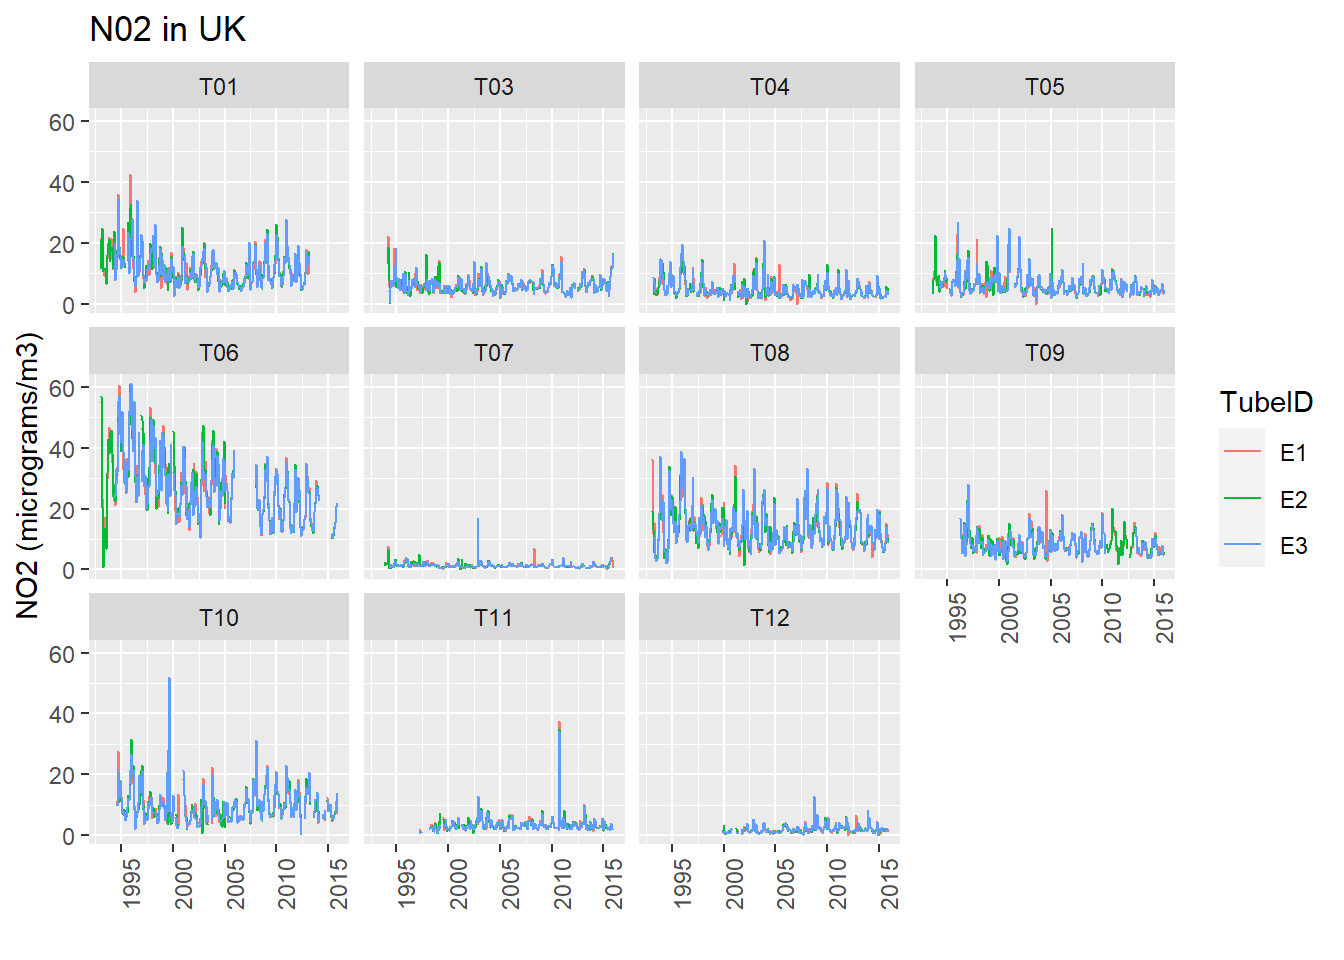
\includegraphics{lec_10_hmm_files/figure-beamer/unnamed-chunk-4-1} \end{center}

\end{frame}

\begin{frame}{HMM theory}
\protect\hypertarget{hmm-theory-2}{}

Matrix \(\Gamma\) is the 1-step transitions. However k-step transition
probabilities can be generated,

\(\Gamma(k) = \Gamma^{k}\)

\begin{itemize}
\tightlist
\item
  From this, we can also calculate the stationary distribution of the
  chain

  \begin{itemize}
  \tightlist
  \item
    See Zucchini et al.~(2006) Chapter 2
  \end{itemize}
\end{itemize}

\end{frame}

\begin{frame}{HMM theory}
\protect\hypertarget{hmm-theory-3}{}

There are two general flavours of transition matrices:

\begin{itemize}
\tightlist
\item
  Homogenous (or stationary)

  \begin{itemize}
  \tightlist
  \item
    transition probabilities don't depend on \(t\)
  \end{itemize}
\item
  Non-homogeneous

  \begin{itemize}
  \tightlist
  \item
    transition probabilities are time-varying
  \end{itemize}
\item
  In this class, we'll mostly consider \textbf{homogeneous} cases
\end{itemize}

\end{frame}

\begin{frame}{HMM theory}
\protect\hypertarget{hmm-theory-4}{}

Covariates may enter HMMs in one of two ways

\begin{itemize}
\item
  Effects on the mean
\item
  Effects on the transition matrix \(\Gamma\)
\item
  For effects on \(\Gamma\), probabilities are constrained (0,1) and
  constrained to sum to 1

  \begin{itemize}
  \tightlist
  \item
    multivariate logit regression used to relate covariates to elements
    of \(\Gamma\)
  \item
    reference / base case is fixed at zero (Agresti 2002)
  \end{itemize}
\end{itemize}

\end{frame}

\begin{frame}[fragile]{HMMs theory}
\protect\hypertarget{hmms-theory-2}{}

\begin{itemize}
\tightlist
\item
  Returning to our simulation example, let's include a temporal trend in
  the transition probabilities
\item
  We assume trend is linear in logit space
\item
  For simplicity, we assume that slope is same on \({ \gamma }_{ 12 }\)
  and \({ \gamma }_{ 21 }\)
\end{itemize}

\begin{Shaded}
\begin{Highlighting}[]
\KeywordTok{plogis}\NormalTok{(}\KeywordTok{logit}\NormalTok{(}\FloatTok{0.1}\NormalTok{) }\OperatorTok{+}\StringTok{ }\FloatTok{0.015}\OperatorTok{*}\DecValTok{1}\OperatorTok{:}\DecValTok{100}\NormalTok{)}
\end{Highlighting}
\end{Shaded}

\begin{center}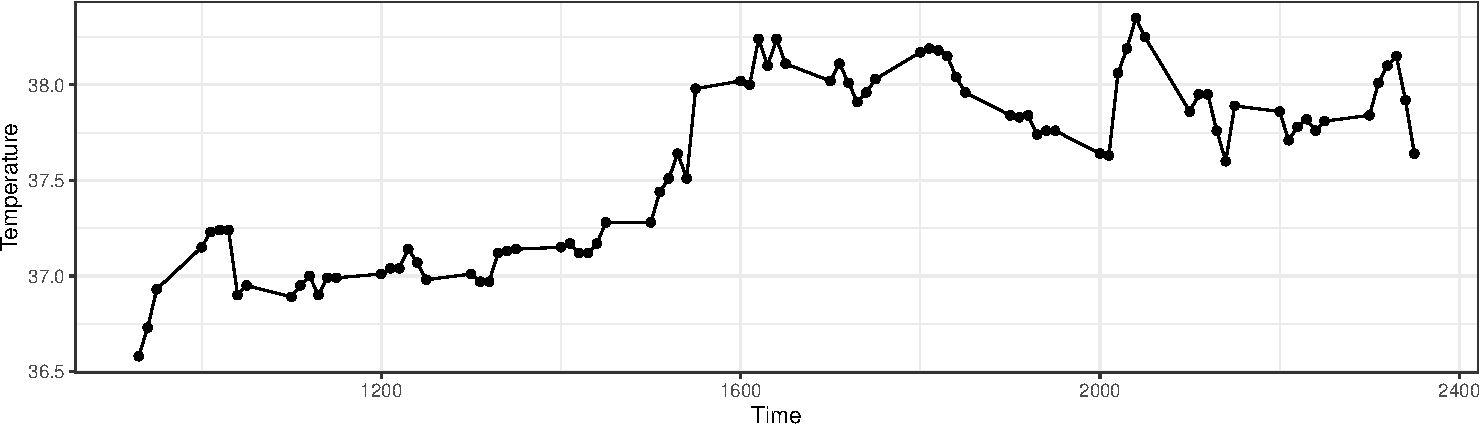
\includegraphics{lec_10_hmm_files/figure-beamer/unnamed-chunk-6-1} \end{center}

\end{frame}

\begin{frame}[fragile]{HMMs theory}
\protect\hypertarget{hmms-theory-3}{}

\begin{Shaded}
\begin{Highlighting}[]
\CommentTok{# initial state}
\NormalTok{x <-}\StringTok{ }\KeywordTok{sample}\NormalTok{(}\DecValTok{1}\OperatorTok{:}\DecValTok{2}\NormalTok{, }\DataTypeTok{size=}\DecValTok{1}\NormalTok{)}
\CommentTok{# transition matrix}
\NormalTok{Gamma =}\StringTok{ }\KeywordTok{matrix}\NormalTok{(}\KeywordTok{c}\NormalTok{(}\FloatTok{0.9}\NormalTok{,}\FloatTok{0.1}\NormalTok{,}\FloatTok{0.2}\NormalTok{,}\FloatTok{0.8}\NormalTok{),}\DecValTok{2}\NormalTok{,}\DecValTok{2}\NormalTok{)}
\ControlFlowTok{for}\NormalTok{(t }\ControlFlowTok{in} \DecValTok{2}\OperatorTok{:}\DecValTok{100}\NormalTok{) \{}
\NormalTok{  Gamma[}\DecValTok{1}\NormalTok{,}\DecValTok{2}\NormalTok{] =}\StringTok{ }\KeywordTok{plogis}\NormalTok{(}\KeywordTok{logit}\NormalTok{(}\FloatTok{0.1}\NormalTok{) }\OperatorTok{+}\StringTok{ }\FloatTok{0.015}\OperatorTok{*}\NormalTok{t)}
\NormalTok{  Gamma[}\DecValTok{1}\NormalTok{,}\DecValTok{1}\NormalTok{] =}\StringTok{ }\DecValTok{1} \OperatorTok{-}\StringTok{ }\NormalTok{Gamma[}\DecValTok{1}\NormalTok{,}\DecValTok{2}\NormalTok{]}
\NormalTok{  Gamma[}\DecValTok{2}\NormalTok{,}\DecValTok{1}\NormalTok{] =}\StringTok{ }\KeywordTok{plogis}\NormalTok{(}\KeywordTok{logit}\NormalTok{(}\FloatTok{0.2}\NormalTok{) }\OperatorTok{+}\StringTok{ }\FloatTok{0.015}\OperatorTok{*}\NormalTok{t)}
\NormalTok{  Gamma[}\DecValTok{2}\NormalTok{,}\DecValTok{2}\NormalTok{] =}\StringTok{ }\DecValTok{1} \OperatorTok{-}\StringTok{ }\NormalTok{Gamma[}\DecValTok{2}\NormalTok{,}\DecValTok{1}\NormalTok{]}
\NormalTok{  x[t] <-}\StringTok{ }\KeywordTok{sample}\NormalTok{(}\DecValTok{1}\OperatorTok{:}\DecValTok{2}\NormalTok{, }\DataTypeTok{size=}\DecValTok{1}\NormalTok{,}\DataTypeTok{prob =}\NormalTok{ Gamma[x[t}\DecValTok{-1}\NormalTok{],])}
\NormalTok{\}}
\end{Highlighting}
\end{Shaded}

\end{frame}

\begin{frame}{HMMs theory}
\protect\hypertarget{hmms-theory-4}{}

\begin{center}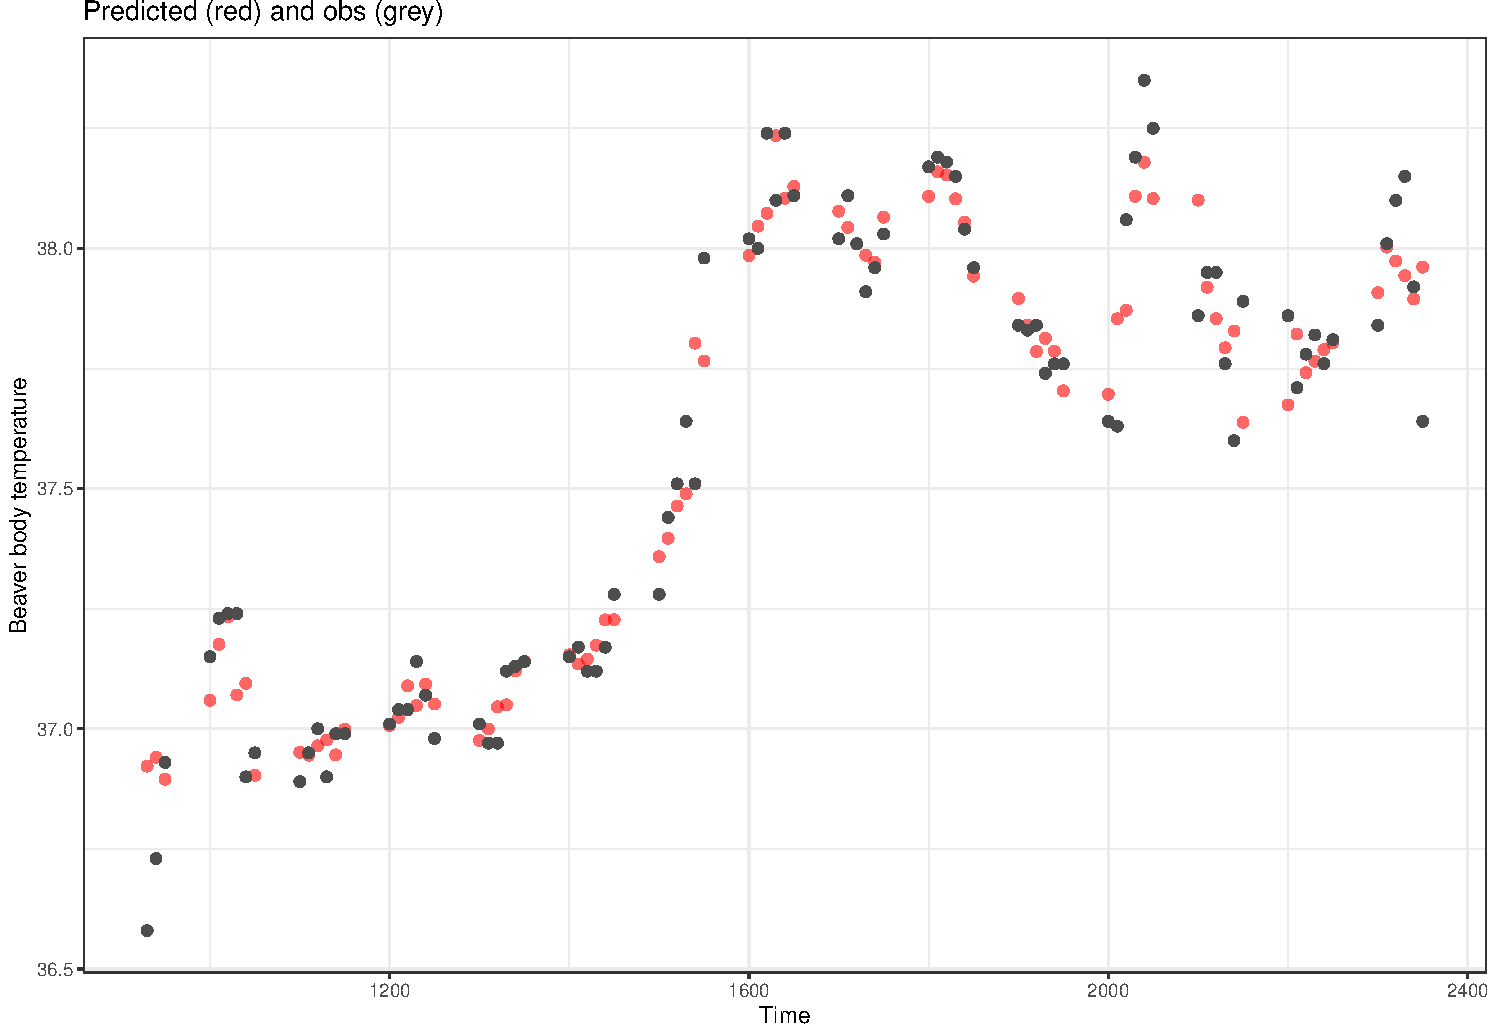
\includegraphics{lec_10_hmm_files/figure-beamer/unnamed-chunk-8-1} \end{center}

\end{frame}

\begin{frame}{HMM: theory}
\protect\hypertarget{hmm-theory-5}{}

\begin{itemize}
\item
  Observations: observable data \({Y}_{ i=1,...,N }\)
\item
  States: latent (discrete) variables that are not directly observed

  \begin{itemize}
  \tightlist
  \item
    \({x}_{ t=1,...,T }\)
  \item
    \(N\) is the number of states possible
  \end{itemize}
\item
  Transition probabilities: transition matrix representing the
  probability of transitioning between states in the Markov chain

  \begin{itemize}
  \tightlist
  \item
    \(\Gamma\) and \({ \gamma }_{ ij }\)
  \end{itemize}
\item
  Emission probabilities: how likely the states are at any particular
  timestep

  \begin{itemize}
  \tightlist
  \item
    \({ \theta }_{ i=1,...,N }\)
  \end{itemize}
\end{itemize}

\end{frame}

\begin{frame}[fragile]{HMM: theory}
\protect\hypertarget{hmm-theory-6}{}

\begin{itemize}
\tightlist
\item
  Our simulations haven't yet included an observation component. Let's
  add observed data that's normally distributed
\end{itemize}

\begin{Shaded}
\begin{Highlighting}[]
\CommentTok{# initial state}
\NormalTok{x <-}\StringTok{ }\KeywordTok{sample}\NormalTok{(}\DecValTok{1}\OperatorTok{:}\DecValTok{2}\NormalTok{, }\DataTypeTok{size=}\DecValTok{1}\NormalTok{)}
\CommentTok{# transition matrix}
\NormalTok{Gamma =}\StringTok{ }\KeywordTok{matrix}\NormalTok{(}\KeywordTok{c}\NormalTok{(}\FloatTok{0.9}\NormalTok{,}\FloatTok{0.1}\NormalTok{,}\FloatTok{0.2}\NormalTok{,}\FloatTok{0.8}\NormalTok{),}\DecValTok{2}\NormalTok{,}\DecValTok{2}\NormalTok{)}
\ControlFlowTok{for}\NormalTok{(t }\ControlFlowTok{in} \DecValTok{2}\OperatorTok{:}\DecValTok{100}\NormalTok{) \{}
\NormalTok{  x[t] <-}\StringTok{ }\KeywordTok{sample}\NormalTok{(}\DecValTok{1}\OperatorTok{:}\DecValTok{2}\NormalTok{, }\DataTypeTok{size=}\DecValTok{1}\NormalTok{,}\DataTypeTok{prob =}\NormalTok{ Gamma[x[t}\DecValTok{-1}\NormalTok{],])}
\NormalTok{\}}

\NormalTok{u =}\StringTok{ }\KeywordTok{c}\NormalTok{(}\FloatTok{1.2}\NormalTok{, }\FloatTok{5.4}\NormalTok{)}
\NormalTok{y =}\StringTok{ }\KeywordTok{rnorm}\NormalTok{(}\KeywordTok{length}\NormalTok{(x), u[x], }\DecValTok{1}\NormalTok{)}
\end{Highlighting}
\end{Shaded}

\end{frame}

\begin{frame}{HMM: theory}
\protect\hypertarget{hmm-theory-7}{}

\begin{center}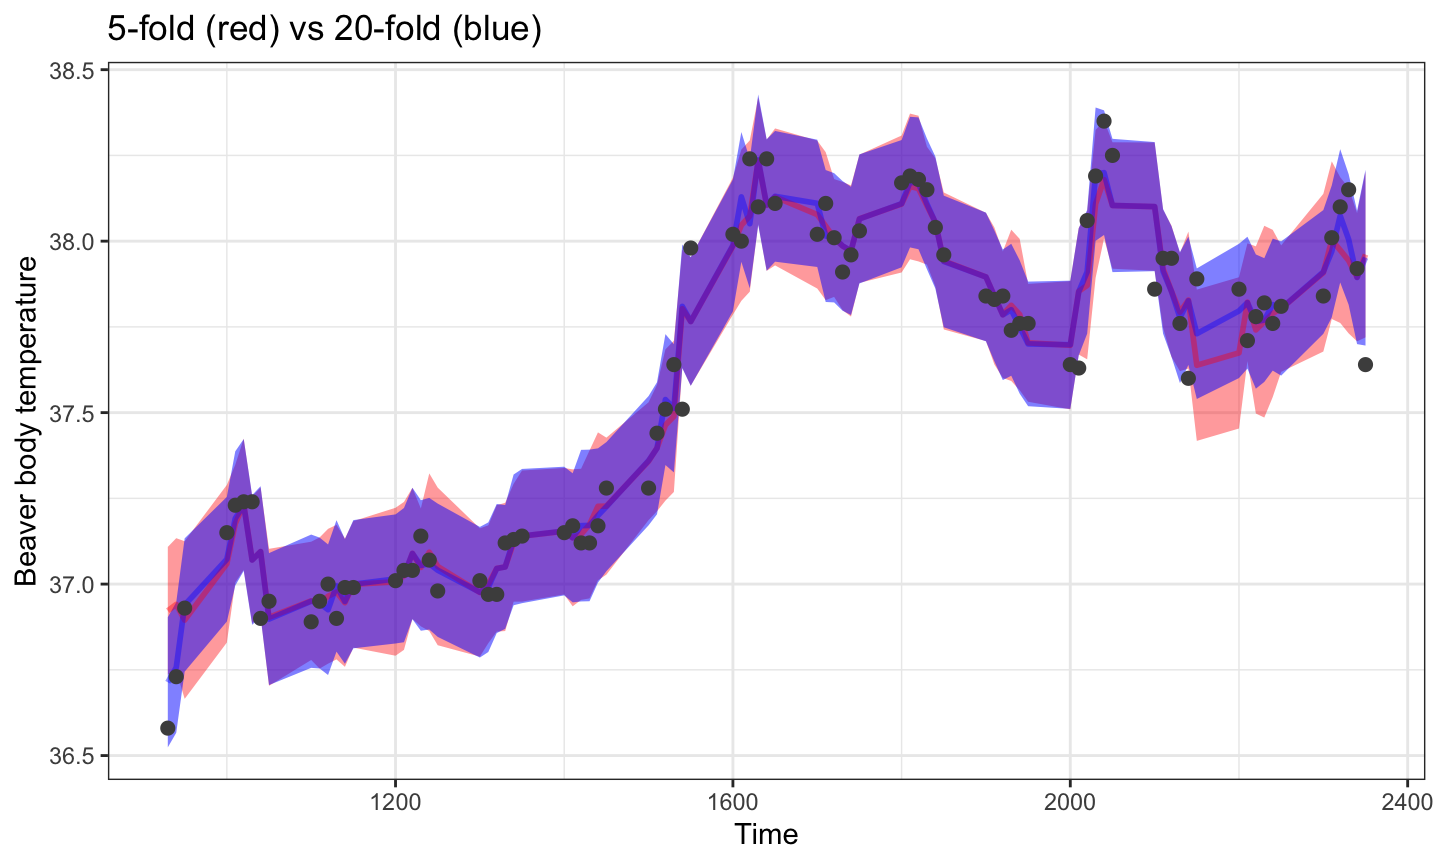
\includegraphics{lec_10_hmm_files/figure-beamer/unnamed-chunk-10-1} \end{center}

\end{frame}

\begin{frame}{HMM: theory}
\protect\hypertarget{hmm-theory-8}{}

One quantity of interest from HMMs is the marginal distribution,
\(P(Y_{t})\)

Output from the model will give us the conditional distribution,
\(P(Y_{t}|x_{t}=i)\). But we need to marginalize over all possible
states

Solution:
\[P(Y_{ t })=\sum _{ i=1 }^{ N }{ P({ x }_{ t }=i)P({ Y }_{ t }|{ x }_{ t }=i) }\]
which can also be expressed as
\[P(Y_{ t })=\sum _{ i=1 }^{ N }{ { \delta  }_{ i }P({ Y }_{ t }|{ x }_{ t }=i) }\]
where \(\delta\) represents the stationary distribution (Zucchini et
al.~2006)

\end{frame}

\begin{frame}{HMM: theory}
\protect\hypertarget{hmm-theory-9}{}

Estimation of HMM parameters can be quite complicated

Dealing with joint likelihood of observed data and unobserved states

\[P(x,Y)=\prod _{ i=1 }^{ T }{ P({ x }_{ t }|{ x }_{ t-1 })P({ Y }_{ t }|{ x }_{ t }) }\]

\end{frame}

\begin{frame}{HMM: theory}
\protect\hypertarget{hmm-theory-10}{}

Estimation most commonly done with maximum likelihood

\begin{enumerate}
\tightlist
\item
  Forward-backward algorithm: calculate probability of observed data
  sequence
\item
  Viterbi algorithm: used to generate most likely states
\item
  EM-algorithm: estimate / update parameters
\end{enumerate}

\begin{itemize}
\tightlist
\item
  For forward-backward algorithm we can factor conditional state
  probabilties
\end{itemize}

\[P\left( { x }_{ t }|{ Y }_{ 1:T } \right) =P({ x }_{ t }|{ Y }_{ 1:t },{ Y }_{ t+1:T })=P({ x }_{ t }|{ Y }_{ 1:t })P({ Y }_{ t+1:T }|{ x }_{ t })\]
* Probability of state given the data is the probability of the state
given the data up to that time step multiplied by the probability of
future data given state

\end{frame}

\begin{frame}{HMM: theory}
\protect\hypertarget{hmm-theory-11}{}

Forward-backward algorithm has 3 steps (sometimes 2/3 combined):

\begin{enumerate}
\tightlist
\item
  Forward probabilities
\end{enumerate}

\begin{itemize}
\tightlist
\item
  from the last slide, this step calculates
  \(P({ x }_{ t }|{ Y }_{ 1:t })\)
\end{itemize}

\begin{enumerate}
\setcounter{enumi}{1}
\tightlist
\item
  Backward probabilities
\end{enumerate}

\begin{itemize}
\tightlist
\item
  from the last slide, this step calculates
  \(P({ Y }_{ t+1:T }|{ x }_{ t })\)
\end{itemize}

\begin{enumerate}
\setcounter{enumi}{2}
\tightlist
\item
  Smoothing
\end{enumerate}

\begin{itemize}
\tightlist
\item
  compute marginal likelihood of sequence of state variables
  \(P(x_{t}|Y)\)
\end{itemize}

\end{frame}

\begin{frame}{Examples of univariate HMMs in R}
\protect\hypertarget{examples-of-univariate-hmms-in-r}{}

As a first example, let's use an example of rainfall data in Seattle
from the end of 2018 and beginning of 2019 (accessed from
wunderground.com)

\begin{center}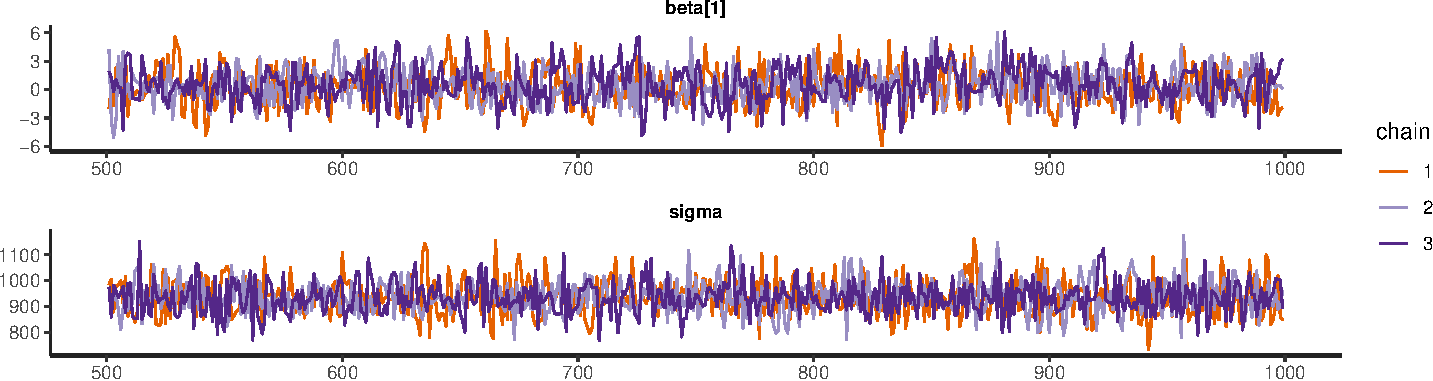
\includegraphics{lec_10_hmm_files/figure-beamer/unnamed-chunk-11-1} \end{center}

\end{frame}

\begin{frame}[fragile]{Examples of univariate HMMs in R}
\protect\hypertarget{examples-of-univariate-hmms-in-r-1}{}

We could model rainfall directly, but for starters let's just model
whether or not it rained on a given day (0/1).

\begin{Shaded}
\begin{Highlighting}[]
\NormalTok{rain}\OperatorTok{$}\NormalTok{rained =}\StringTok{ }\KeywordTok{ifelse}\NormalTok{(rain}\OperatorTok{$}\NormalTok{Rainfall }\OperatorTok{>}\StringTok{ }\DecValTok{0}\NormalTok{, }\DecValTok{1}\NormalTok{, }\DecValTok{0}\NormalTok{)}
\end{Highlighting}
\end{Shaded}

\begin{center}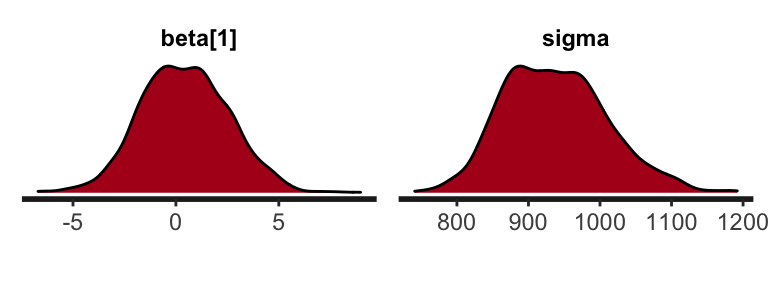
\includegraphics{lec_10_hmm_files/figure-beamer/unnamed-chunk-13-1} \end{center}

\end{frame}

\begin{frame}{Examples of univariate HMMs in R}
\protect\hypertarget{examples-of-univariate-hmms-in-r-2}{}

Questions that we might be interested in:

\begin{itemize}
\tightlist
\item
  Conditional probabilities

  \begin{itemize}
  \tightlist
  \item
    What's the probability of it raining tomorrow given that it's
    raining today?
  \item
    What's the probability of it raining tomorrow given that it's not
    today?
  \end{itemize}
\item
  Persistence

  \begin{itemize}
  \tightlist
  \item
    On average, how long might we expect to go without rain?
  \end{itemize}
\end{itemize}

\end{frame}

\begin{frame}{Examples of univariate HMMs in R}
\protect\hypertarget{examples-of-univariate-hmms-in-r-3}{}

We don't really need HMMs to address these questions

\begin{itemize}
\tightlist
\item
  daily rainfall may be measured with a tiny amount of uncertainty
\item
  probably safe to say that there's almost no uncertainty in whether or
  not it rained on a given day
\end{itemize}

\end{frame}

\begin{frame}[fragile]{Examples of univariate HMMs in R}
\protect\hypertarget{examples-of-univariate-hmms-in-r-4}{}

Transition probabilities can be just calculated directly,

\begin{itemize}
\tightlist
\item
  \(P(rain_{t+1} | rain_{t})\)
\end{itemize}

\[\frac { \# consecutive \quad rainy \quad days }{ \# rainy \quad days }\]

For example, we can create a differenced variable to indicate no change
(0), and compute

\begin{Shaded}
\begin{Highlighting}[]
\NormalTok{rain}\OperatorTok{$}\NormalTok{diff =}\StringTok{ }\KeywordTok{c}\NormalTok{(}\KeywordTok{diff}\NormalTok{(rain}\OperatorTok{$}\NormalTok{rained), }\OtherTok{NA}\NormalTok{)}
\NormalTok{p_rain_rain =}\StringTok{ }\KeywordTok{length}\NormalTok{(}\KeywordTok{which}\NormalTok{(rain}\OperatorTok{$}\NormalTok{diff }\OperatorTok{==}\StringTok{ }\DecValTok{0} \OperatorTok{&}\StringTok{ }
\StringTok{    }\NormalTok{rain}\OperatorTok{$}\NormalTok{rained}\OperatorTok{==}\DecValTok{1}\NormalTok{)) }\OperatorTok{/}\StringTok{ }\KeywordTok{length}\NormalTok{(}\KeywordTok{which}\NormalTok{(rain}\OperatorTok{$}\NormalTok{rained}\OperatorTok{==}\DecValTok{1}\NormalTok{))}
\end{Highlighting}
\end{Shaded}

\end{frame}

\begin{frame}[fragile]{Examples of univariate HMMs in R}
\protect\hypertarget{examples-of-univariate-hmms-in-r-5}{}

Ok, now let's assume that there's some minor observation or measurement
error in the rain gauge data. For this case, it's best to use a HMM.

Let's start with using the R package \texttt{depmixS4}. There's a good
vignette on the package that you can refer back to,

\url{https://cran.r-project.org/web/packages/depmixS4/vignettes/depmixS4.pdf}

\end{frame}

\begin{frame}[fragile]{Examples of univariate HMMs in R}
\protect\hypertarget{examples-of-univariate-hmms-in-r-6}{}

There's two functions we'll use to set up the HMM with
\texttt{depmixS4}.

First we'll structure the model using the same formula notation you're
hopefully familiar with,

\begin{Shaded}
\begin{Highlighting}[]
\NormalTok{mod =}\StringTok{ }\KeywordTok{depmix}\NormalTok{(rained }\OperatorTok{~}\StringTok{ }\DecValTok{1}\NormalTok{, }
             \DataTypeTok{nstates =} \DecValTok{2}\NormalTok{, }
             \DataTypeTok{transition =} \OperatorTok{~}\StringTok{ }\DecValTok{1}\NormalTok{,}
             \DataTypeTok{family =} \KeywordTok{binomial}\NormalTok{(),}
             \DataTypeTok{data=}\NormalTok{rain)}
\end{Highlighting}
\end{Shaded}

\end{frame}

\begin{frame}[fragile]{Examples of univariate HMMs in R}
\protect\hypertarget{examples-of-univariate-hmms-in-r-7}{}

Stepping through this \texttt{rained} is our response (yes / no)

\begin{Shaded}
\begin{Highlighting}[]
\NormalTok{mod =}\StringTok{ }\KeywordTok{depmix}\NormalTok{(rained }\OperatorTok{~}\StringTok{ }\DecValTok{1}\NormalTok{, }
             \DataTypeTok{nstates =} \DecValTok{2}\NormalTok{, }
             \DataTypeTok{transition =} \OperatorTok{~}\StringTok{ }\DecValTok{1}\NormalTok{,}
             \DataTypeTok{family =} \KeywordTok{binomial}\NormalTok{(),}
             \DataTypeTok{data=}\NormalTok{rain)}
\end{Highlighting}
\end{Shaded}

\end{frame}

\begin{frame}[fragile]{Examples of univariate HMMs in R}
\protect\hypertarget{examples-of-univariate-hmms-in-r-8}{}

\texttt{nstates} is the number of alternative states (\textgreater{} 2),
specified a priori

\begin{Shaded}
\begin{Highlighting}[]
\NormalTok{mod =}\StringTok{ }\KeywordTok{depmix}\NormalTok{(rained }\OperatorTok{~}\StringTok{ }\DecValTok{1}\NormalTok{, }
             \DataTypeTok{nstates =} \DecValTok{2}\NormalTok{, }
             \DataTypeTok{transition =} \OperatorTok{~}\StringTok{ }\DecValTok{1}\NormalTok{,}
             \DataTypeTok{family =} \KeywordTok{binomial}\NormalTok{(),}
             \DataTypeTok{data=}\NormalTok{rain)}
\end{Highlighting}
\end{Shaded}

\end{frame}

\begin{frame}[fragile]{Examples of univariate HMMs in R}
\protect\hypertarget{examples-of-univariate-hmms-in-r-9}{}

\texttt{transition} is a formula to specify whether any covariates are
to be included in the transition probabilities. The default is no
covariates, and that these transitions aren't time varying.

\begin{Shaded}
\begin{Highlighting}[]
\NormalTok{mod =}\StringTok{ }\KeywordTok{depmix}\NormalTok{(rained }\OperatorTok{~}\StringTok{ }\DecValTok{1}\NormalTok{, }
             \DataTypeTok{nstates =} \DecValTok{2}\NormalTok{, }
             \DataTypeTok{transition =} \OperatorTok{~}\StringTok{ }\DecValTok{1}\NormalTok{,}
             \DataTypeTok{family =} \KeywordTok{binomial}\NormalTok{(),}
             \DataTypeTok{data=}\NormalTok{rain)}
\end{Highlighting}
\end{Shaded}

\end{frame}

\begin{frame}[fragile]{Examples of univariate HMMs in R}
\protect\hypertarget{examples-of-univariate-hmms-in-r-10}{}

\texttt{family} is family or list of families (a list for multiple
response variables) of the families associated with each response. The
majority of common families are supported

\begin{Shaded}
\begin{Highlighting}[]
\NormalTok{mod =}\StringTok{ }\KeywordTok{depmix}\NormalTok{(rained }\OperatorTok{~}\StringTok{ }\DecValTok{1}\NormalTok{, }
             \DataTypeTok{nstates =} \DecValTok{2}\NormalTok{, }
             \DataTypeTok{transition =} \OperatorTok{~}\StringTok{ }\DecValTok{1}\NormalTok{,}
             \DataTypeTok{family =} \KeywordTok{binomial}\NormalTok{(), }
             \DataTypeTok{data=}\NormalTok{rain)}
\end{Highlighting}
\end{Shaded}

For a complete list, see

\begin{Shaded}
\begin{Highlighting}[]
\NormalTok{?depmixS4}\OperatorTok{::}\NormalTok{GLMresponse}
\end{Highlighting}
\end{Shaded}

\end{frame}

\begin{frame}[fragile]{Examples of univariate HMMs in R}
\protect\hypertarget{examples-of-univariate-hmms-in-r-11}{}

Ok, now that we've set up the model, we can do the estimation and look
at the output

\begin{Shaded}
\begin{Highlighting}[]
\KeywordTok{set.seed}\NormalTok{(}\DecValTok{123}\NormalTok{)}
\NormalTok{fitmod =}\StringTok{ }\KeywordTok{fit}\NormalTok{(mod)}
\end{Highlighting}
\end{Shaded}

\begin{longtable}[]{@{}lrr@{}}
\toprule
& To\_1 & To\_2\tabularnewline
\midrule
\endhead
From\_1 & 0.77 & 0.23\tabularnewline
From\_2 & 0.41 & 0.59\tabularnewline
\bottomrule
\end{longtable}

\end{frame}

\begin{frame}[fragile]{Examples of univariate HMMs in R}
\protect\hypertarget{examples-of-univariate-hmms-in-r-12}{}

As a warning, note that the results from the estimation are a bit
sensitive to the initial seed. Look at how much the transition
probabilties change,

\begin{Shaded}
\begin{Highlighting}[]
\KeywordTok{set.seed}\NormalTok{(}\DecValTok{121}\NormalTok{)}
\NormalTok{fitmod =}\StringTok{ }\KeywordTok{fit}\NormalTok{(mod)}
\end{Highlighting}
\end{Shaded}

\begin{longtable}[]{@{}lrr@{}}
\toprule
& To\_1 & To\_2\tabularnewline
\midrule
\endhead
From\_1 & 0.59 & 0.41\tabularnewline
From\_2 & 0.23 & 0.77\tabularnewline
\bottomrule
\end{longtable}

\end{frame}

\begin{frame}{Examples of univariate HMMs in R}
\protect\hypertarget{examples-of-univariate-hmms-in-r-13}{}

There's a couple practical ways to try to overcome this seed issue.

\begin{itemize}
\tightlist
\item
  First, we can change the control parameters
\end{itemize}

\emph{Unfortunately for this example, this doesn't solve the issue}

\end{frame}

\begin{frame}[fragile]{Examples of univariate HMMs in R}
\protect\hypertarget{examples-of-univariate-hmms-in-r-14}{}

\begin{itemize}
\tightlist
\item
  A second option is to run the estimation across a large number
  (\textgreater{} 100) of random starting values
\end{itemize}

Pseudocode:

\begin{Shaded}
\begin{Highlighting}[]
\NormalTok{best =}\StringTok{ }\FloatTok{1.0e10}
\NormalTok{best_model =}\StringTok{ }\OtherTok{NA}
\ControlFlowTok{for}\NormalTok{(i }\ControlFlowTok{in} \DecValTok{1}\OperatorTok{:}\NormalTok{iter) \{}
  \CommentTok{# fit the model}
\NormalTok{  fitmod =}\StringTok{ }\KeywordTok{fit}\NormalTok{(mod)}
  
  \CommentTok{# check to see if this is the best solution?}
  \ControlFlowTok{if}\NormalTok{(}\KeywordTok{AIC}\NormalTok{(fitmod) }\OperatorTok{<}\StringTok{ }\NormalTok{best) \{}
\NormalTok{    best_model =}\StringTok{ }\NormalTok{fitmod}
\NormalTok{    best =}\StringTok{ }\KeywordTok{AIC}\NormalTok{(fitmod)}
\NormalTok{  \}}
\NormalTok{\}}
\end{Highlighting}
\end{Shaded}

\end{frame}

\begin{frame}{Examples of univariate HMMs in R}
\protect\hypertarget{examples-of-univariate-hmms-in-r-15}{}

Let's move on to a more complex example.

We'll pull some data from the CalCOFI ichthyoplankton cruises in
Southern California. Some species have been used to indicate \emph{cool}
versus \emph{warm} regimes.

\begin{itemize}
\tightlist
\item
  \url{http://calcofi.org/publications/calcofireports/v58/Vol58-State_of_the_Current_pages_1-55.pdf}
\end{itemize}

For this example, we'll focus on the California smoothtongue
(\emph{Leuroglossus stilbius})

\end{frame}

\begin{frame}{Examples of univariate HMMs in R}
\protect\hypertarget{examples-of-univariate-hmms-in-r-16}{}

\emph{Caveat:} the survey is spatially gridded, and you'd want to
perform index standardization or use spatial models to generate indices.
For simplicty, we're just taking the mean abundance across stations in
April-May.

\begin{center}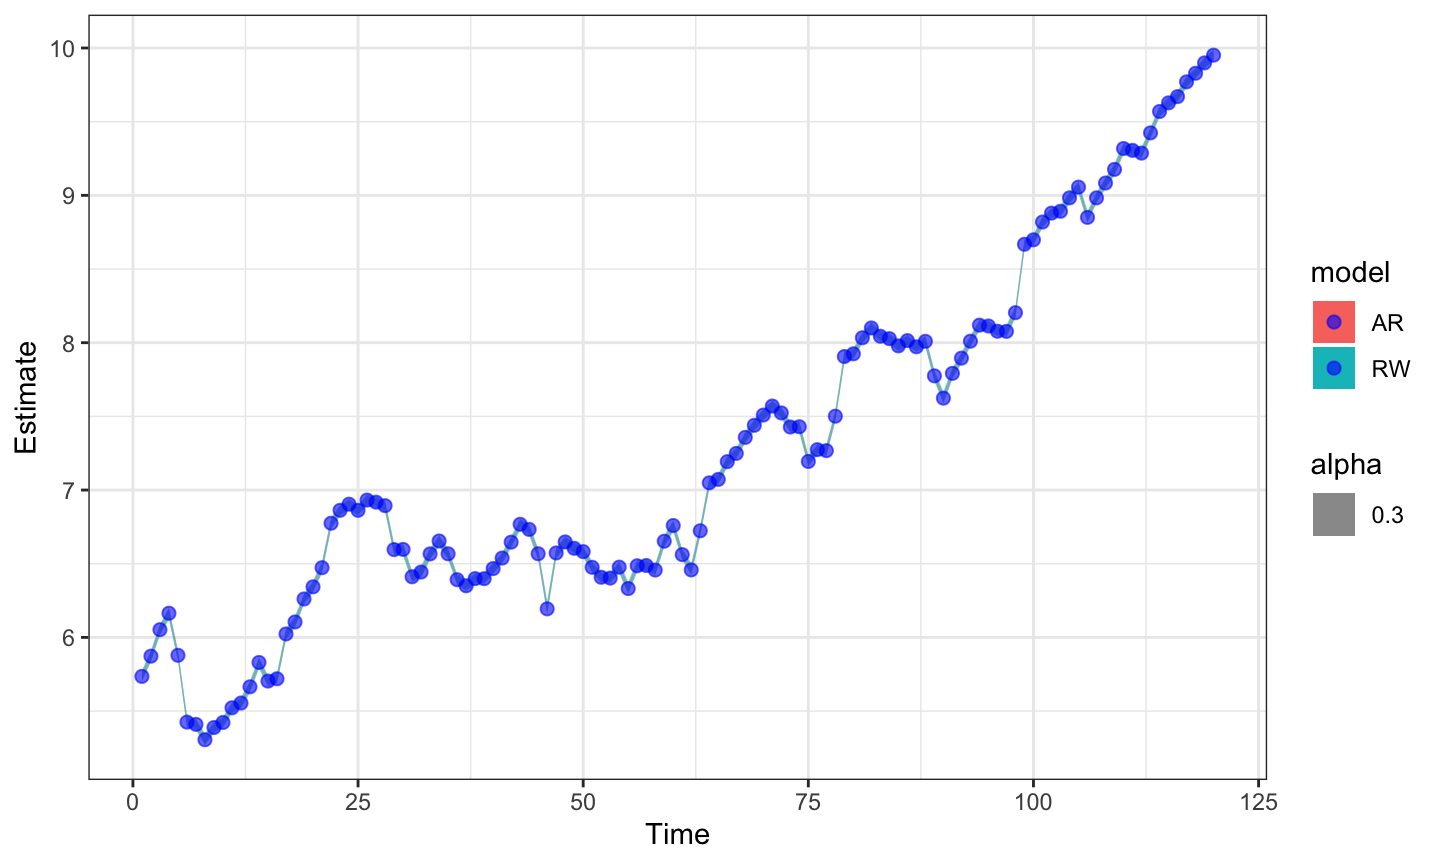
\includegraphics{lec_10_hmm_files/figure-beamer/unnamed-chunk-29-1} \end{center}

\end{frame}

\begin{frame}[fragile]{Examples of univariate HMMs in R}
\protect\hypertarget{examples-of-univariate-hmms-in-r-17}{}

We'll start with fitting a 2-state model with \texttt{depmix}.
Assumptions:

\begin{itemize}
\tightlist
\item
  Model fit to ln transformed data, assumed Gaussian
\end{itemize}

\begin{Shaded}
\begin{Highlighting}[]
\KeywordTok{set.seed}\NormalTok{(}\DecValTok{123}\NormalTok{)}
\NormalTok{calcofi}\OperatorTok{$}\NormalTok{ln =}\StringTok{ }\KeywordTok{log}\NormalTok{(calcofi}\OperatorTok{$}\NormalTok{m)}
\NormalTok{mod =}\StringTok{ }\KeywordTok{depmix}\NormalTok{(ln }\OperatorTok{~}\StringTok{ }\DecValTok{1}\NormalTok{, }
             \DataTypeTok{nstates =} \DecValTok{2}\NormalTok{, }
             \DataTypeTok{data=}\NormalTok{calcofi)}
\NormalTok{fitmod =}\StringTok{ }\KeywordTok{fit}\NormalTok{(mod)}
\end{Highlighting}
\end{Shaded}

\end{frame}

\begin{frame}[fragile]{Examples of univariate HMMs in R}
\protect\hypertarget{examples-of-univariate-hmms-in-r-18}{}

First let's look at how to get predictions out of a
\texttt{depmix.fitted} object

We'll start with the state probabilities. Remember we could work with
either

\begin{itemize}
\tightlist
\item
  Most probable state trajectory - via the \texttt{viterbi} function
\item
  Marginals of \(P(x_{t})\) - via the \texttt{posterior} function
\end{itemize}

\end{frame}

\begin{frame}[fragile]{Examples of univariate HMMs in R}
\protect\hypertarget{examples-of-univariate-hmms-in-r-19}{}

The most probable states are

\begin{Shaded}
\begin{Highlighting}[]
\NormalTok{prstates =}\StringTok{ }\KeywordTok{apply}\NormalTok{(}\KeywordTok{posterior}\NormalTok{(fitmod)[,}\KeywordTok{c}\NormalTok{(}\StringTok{"S1"}\NormalTok{,}\StringTok{"S2"}\NormalTok{)], }
  \DecValTok{1}\NormalTok{, which.max)}
\end{Highlighting}
\end{Shaded}

\begin{Shaded}
\begin{Highlighting}[]
\KeywordTok{plot}\NormalTok{(prstates, }\DataTypeTok{type=}\StringTok{"b"}\NormalTok{, }\DataTypeTok{xlab=}\StringTok{"Time"}\NormalTok{, }\DataTypeTok{ylab=}\StringTok{"State"}\NormalTok{)}
\end{Highlighting}
\end{Shaded}

\begin{center}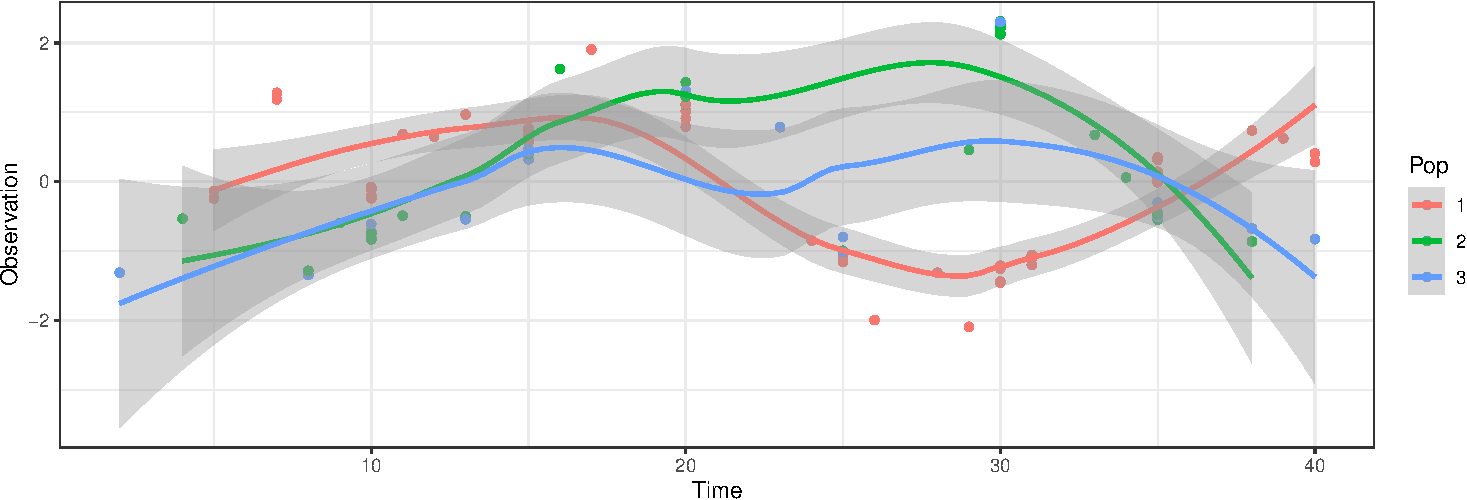
\includegraphics{lec_10_hmm_files/figure-beamer/unnamed-chunk-32-1} \end{center}

\end{frame}

\begin{frame}[fragile]{Examples of univariate HMMs in R}
\protect\hypertarget{examples-of-univariate-hmms-in-r-20}{}

\texttt{depmixS4} doesn't have a \texttt{predict()} or
\texttt{forecast()} function, but creating estimated data is pretty
straightforward. We can get the means out with

\begin{Shaded}
\begin{Highlighting}[]
\NormalTok{mu =}\StringTok{ }\KeywordTok{summary}\NormalTok{(fitmod)[,}\DecValTok{1}\NormalTok{]}
\end{Highlighting}
\end{Shaded}

\begin{Shaded}
\begin{Highlighting}[]
\NormalTok{pred =}\StringTok{ }\KeywordTok{data.frame}\NormalTok{(}\StringTok{"year"}\NormalTok{=}\KeywordTok{seq}\NormalTok{(}\KeywordTok{min}\NormalTok{(calcofi}\OperatorTok{$}\NormalTok{year), }
  \KeywordTok{max}\NormalTok{(calcofi}\OperatorTok{$}\NormalTok{year)),}
  \StringTok{"fit"}\NormalTok{ =}\StringTok{ }\NormalTok{mu[prstates])}
\end{Highlighting}
\end{Shaded}

\begin{center}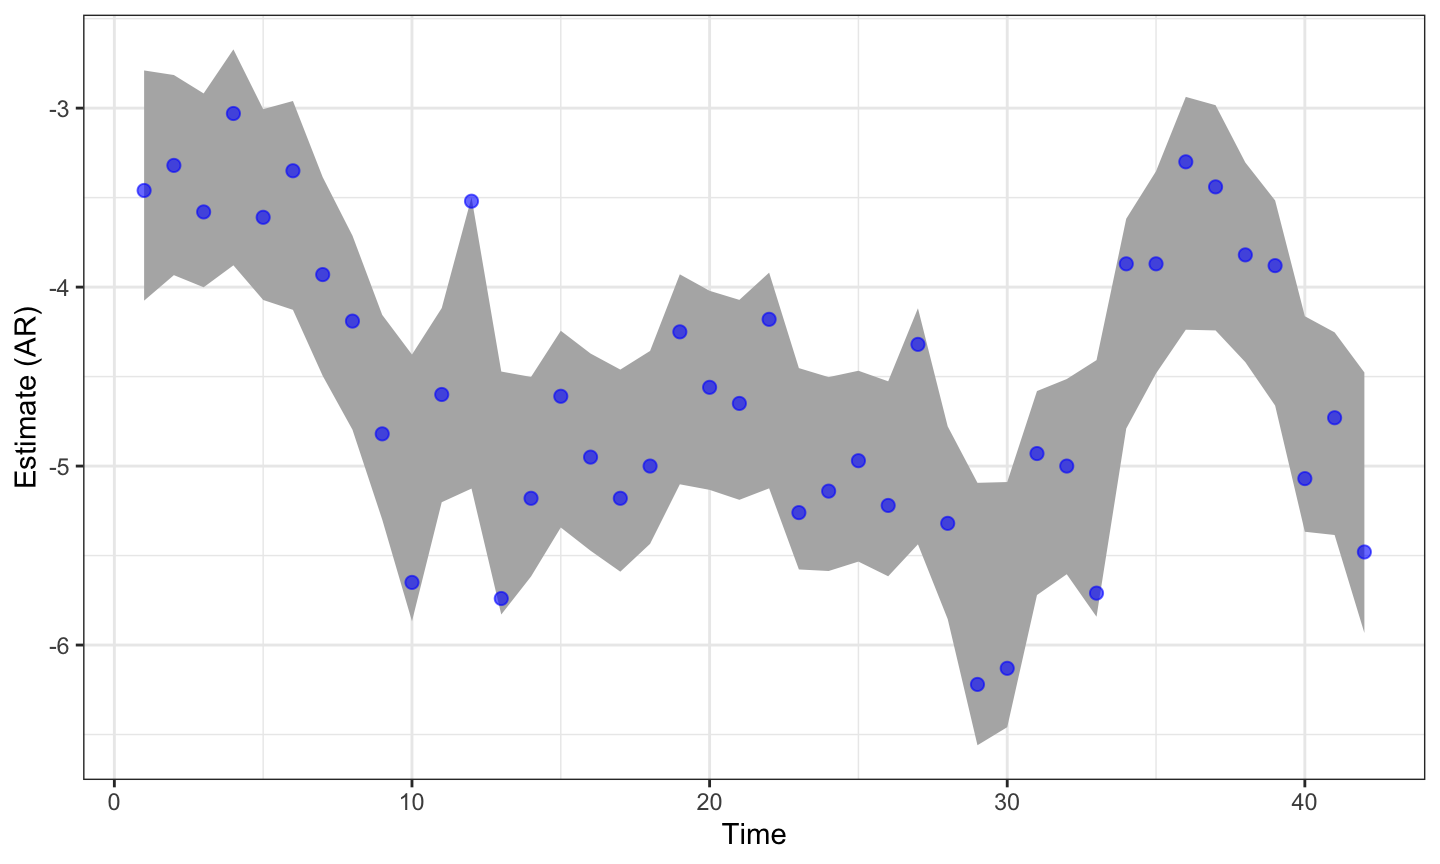
\includegraphics{lec_10_hmm_files/figure-beamer/unnamed-chunk-35-1} \end{center}

\end{frame}

\begin{frame}[fragile]{Examples of univariate HMMs in R}
\protect\hypertarget{examples-of-univariate-hmms-in-r-21}{}

Some diagnostics (like autocorrelation) may not look great. What if we
compared the previous model to one with 3 states? AIC from the 2-state
model was

\begin{verbatim}
## [1] 118.994
\end{verbatim}

\begin{Shaded}
\begin{Highlighting}[]
\KeywordTok{set.seed}\NormalTok{(}\DecValTok{123}\NormalTok{)}
\NormalTok{calcofi}\OperatorTok{$}\NormalTok{ln =}\StringTok{ }\KeywordTok{log}\NormalTok{(calcofi}\OperatorTok{$}\NormalTok{m)}
\NormalTok{mod =}\StringTok{ }\KeywordTok{depmix}\NormalTok{(ln }\OperatorTok{~}\StringTok{ }\DecValTok{1}\NormalTok{, }
             \DataTypeTok{nstates =} \DecValTok{3}\NormalTok{, }
             \DataTypeTok{data=}\NormalTok{calcofi)}
\NormalTok{fitmod =}\StringTok{ }\KeywordTok{fit}\NormalTok{(mod)}
\end{Highlighting}
\end{Shaded}

This seems like increasing the states doesn't result in lower AIC

\begin{verbatim}
## [1] 122.5181
\end{verbatim}

\end{frame}

\begin{frame}{Model selection \& diagnostics}
\protect\hypertarget{model-selection-diagnostics}{}

\begin{itemize}
\item
  In comparing 2 vs 3 state HMM, we found lower AIC for 2-state model
\item
  However, opposite is often true -- more states fit better, and result
  in lower AIC
\item
  How to decide? Occam's razor \& metrics of predictive ability
\item
  Pohle et al.~2017. ``Selecting the Number of States in Hidden Markov
  Models: Pragmatic Solutions Illustrated Using Animal Movement''
\end{itemize}

\end{frame}

\begin{frame}{Examples of multivariate HMMs in R}
\protect\hypertarget{examples-of-multivariate-hmms-in-r}{}

If the univariate examples make sense, it's not that different to extend
these models for multiple time series.

In this setting, the assumption is that the latent state process is the
same for all time series, though the time series may differ

\begin{enumerate}
\tightlist
\item
  their lengths
\item
  their error distributions
\end{enumerate}

\end{frame}

\begin{frame}[fragile]{Examples of multivariate HMMs in R}
\protect\hypertarget{examples-of-multivariate-hmms-in-r-1}{}

In \texttt{depmix}, these arguments generally become lists

We'll extend our CalCOFI example to include 2 species now

\begin{center}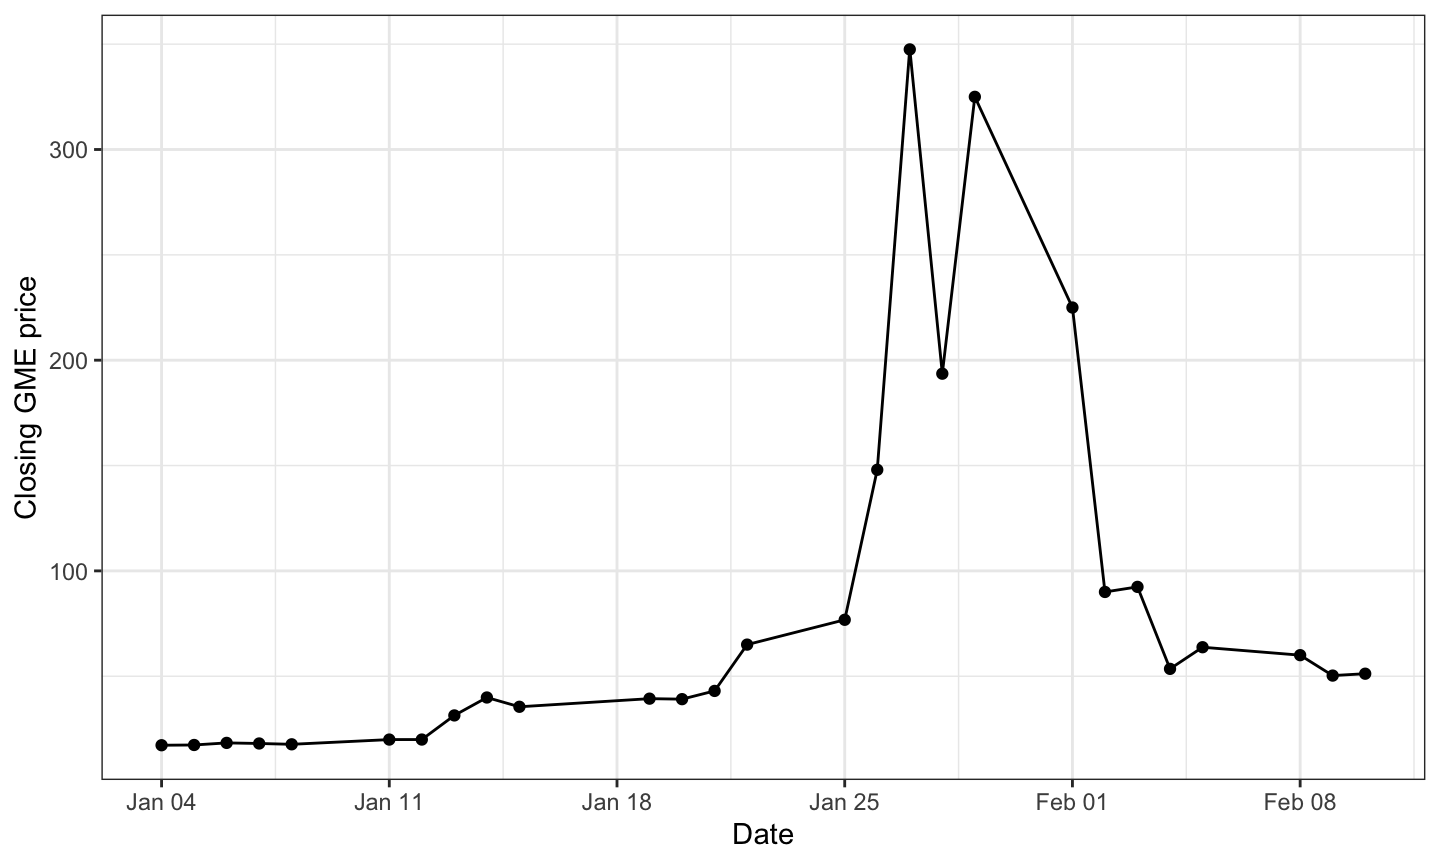
\includegraphics{lec_10_hmm_files/figure-beamer/unnamed-chunk-39-1} \end{center}

\end{frame}

\begin{frame}[fragile]{Examples of multivariate HMMs in R}
\protect\hypertarget{examples-of-multivariate-hmms-in-r-2}{}

Fitting a 2-state model with 2 species as responses. First we have to
reshape the data,

\begin{Shaded}
\begin{Highlighting}[]
\NormalTok{calcofi}\OperatorTok{$}\NormalTok{ln =}\StringTok{ }\KeywordTok{log}\NormalTok{(calcofi}\OperatorTok{$}\NormalTok{m) }\CommentTok{# ln transform}
\NormalTok{calcofi <-}\StringTok{ }\KeywordTok{dcast}\NormalTok{(}\KeywordTok{melt}\NormalTok{(calcofi[,}\KeywordTok{c}\NormalTok{(}\StringTok{"year"}\NormalTok{,}\StringTok{"ln"}\NormalTok{,}\StringTok{"species"}\NormalTok{)], }
            \DataTypeTok{id.vars =} \KeywordTok{c}\NormalTok{(}\StringTok{"year"}\NormalTok{, }\StringTok{"species"}\NormalTok{)), }
\NormalTok{            year }\OperatorTok{~}\StringTok{ }\NormalTok{species)}
\KeywordTok{names}\NormalTok{(calcofi)[}\DecValTok{2}\OperatorTok{:}\DecValTok{3}\NormalTok{] =}\StringTok{ }\KeywordTok{c}\NormalTok{(}\StringTok{"L_stilbius"}\NormalTok{,}\StringTok{"L_ochotensis"}\NormalTok{)}
\KeywordTok{head}\NormalTok{(calcofi)}
\end{Highlighting}
\end{Shaded}

\begin{verbatim}
##   year  L_stilbius L_ochotensis
## 1 1980  0.85449030   -0.8414039
## 2 1981  3.13964169    1.6941728
## 3 1982  3.70359056    3.5435378
## 4 1983 -0.03344793    0.4947281
## 5 1984  3.00082695    2.4346651
## 6 1985  0.24911445   -0.8471716
\end{verbatim}

\end{frame}

\begin{frame}[fragile]{Examples of multivariate HMMs in R}
\protect\hypertarget{examples-of-multivariate-hmms-in-r-3}{}

\begin{Shaded}
\begin{Highlighting}[]
\KeywordTok{set.seed}\NormalTok{(}\DecValTok{123}\NormalTok{)}
\NormalTok{mod =}\StringTok{ }\KeywordTok{depmix}\NormalTok{(}\KeywordTok{list}\NormalTok{(L_stilbius }\OperatorTok{~}\StringTok{ }\DecValTok{1}\NormalTok{, L_ochotensis}\OperatorTok{~}\DecValTok{1}\NormalTok{), }
             \DataTypeTok{nstates =} \DecValTok{2}\NormalTok{, }
             \DataTypeTok{family =} \KeywordTok{list}\NormalTok{(}\KeywordTok{gaussian}\NormalTok{(),}\KeywordTok{gaussian}\NormalTok{()),}
             \DataTypeTok{data=}\NormalTok{calcofi)}
\NormalTok{fitmod =}\StringTok{ }\KeywordTok{fit}\NormalTok{(mod)}
\end{Highlighting}
\end{Shaded}

\end{frame}

\begin{frame}[fragile]{Examples of multivariate HMMs in R}
\protect\hypertarget{examples-of-multivariate-hmms-in-r-4}{}

We could also have situations where the time series are of different
length.

\begin{itemize}
\item
  For example, if L\_ochotensis time series was missing first half of
  values
\item
  The argument \texttt{ntimes} is a list that becomes particularly
  valuable here - representing the length of each time series
\end{itemize}

\end{frame}

\begin{frame}{Summary}
\protect\hypertarget{summary}{}

HMMs are a useful approach at identifying latent state vectors that
undergo discrete transitions

Estimation of HMMs for time series in R generally done with ML methods

\begin{itemize}
\tightlist
\item
  Fast, but these algorithms may get stuck
\item
  Robust solutions = multiple starting values
\end{itemize}

Bayesian estimation generally beyond the scope of this class

\begin{itemize}
\tightlist
\item
  Very straightforward to build these models in BUGS/JAGS
\item
  More complicated with newer sofware (Stan), though examples here:
  \url{https://mc-stan.org/docs/2_26/stan-users-guide/hmms-section.html}
\end{itemize}

\end{frame}

\begin{frame}{JAGS Examples}
\protect\hypertarget{jags-examples}{}

\begin{itemize}
\item
  Why JAGS? Categorical samplers
\item
  Let's re-fit our CalCOFI example in JAGS. We'll step through this in
  small chunks to understand what's going on in JAGS syntax
\end{itemize}

\end{frame}

\begin{frame}[fragile]{JAGS model}
\protect\hypertarget{jags-model}{}

\begin{itemize}
\tightlist
\item
  First we need to specify the initial state. We don't know it, but
  assume each state (1/2) is equally likely
\end{itemize}

\begin{Shaded}
\begin{Highlighting}[]
\NormalTok{model\{}
\ControlFlowTok{for}\NormalTok{(i }\ControlFlowTok{in} \DecValTok{1}\OperatorTok{:}\DecValTok{2}\NormalTok{)\{initp[i] <-}\StringTok{ }\FloatTok{0.5}\NormalTok{\}}
\NormalTok{x[}\DecValTok{1}\NormalTok{] }\OperatorTok{~}\StringTok{ }\KeywordTok{dcat}\NormalTok{(initp)}
\end{Highlighting}
\end{Shaded}

\end{frame}

\begin{frame}[fragile]{JAGS model}
\protect\hypertarget{jags-model-1}{}

\begin{itemize}
\tightlist
\item
  Next we can think about parameterizing the transition matrix.
  \(\Gamma\) is 2 x 2, but only has 2 parameters
\item
  We'll specify uniform(0,1) priors on these
\end{itemize}

\begin{Shaded}
\begin{Highlighting}[]
\NormalTok{model\{}
\ControlFlowTok{for}\NormalTok{(i }\ControlFlowTok{in} \DecValTok{1}\OperatorTok{:}\DecValTok{2}\NormalTok{)\{initp[i] <-}\StringTok{ }\FloatTok{0.5}\NormalTok{\}}
\NormalTok{x[}\DecValTok{1}\NormalTok{] }\OperatorTok{~}\StringTok{ }\KeywordTok{dcat}\NormalTok{(initp)}
\NormalTok{p }\OperatorTok{~}\StringTok{ }\KeywordTok{dunif}\NormalTok{(}\DecValTok{0}\NormalTok{,}\DecValTok{1}\NormalTok{)}
\NormalTok{q }\OperatorTok{~}\StringTok{ }\KeywordTok{dunif}\NormalTok{(}\DecValTok{0}\NormalTok{,}\DecValTok{1}\NormalTok{)}
\end{Highlighting}
\end{Shaded}

\end{frame}

\begin{frame}[fragile]{JAGS model}
\protect\hypertarget{jags-model-2}{}

\begin{itemize}
\tightlist
\item
  Next we specify \(\Gamma\)
\end{itemize}

\begin{Shaded}
\begin{Highlighting}[]
\NormalTok{model\{}
\ControlFlowTok{for}\NormalTok{(i }\ControlFlowTok{in} \DecValTok{1}\OperatorTok{:}\DecValTok{2}\NormalTok{)\{initp[i] <-}\StringTok{ }\FloatTok{0.5}\NormalTok{\}}
\NormalTok{x[}\DecValTok{1}\NormalTok{] }\OperatorTok{~}\StringTok{ }\KeywordTok{dcat}\NormalTok{(initp)}
\NormalTok{gamma12 }\OperatorTok{~}\StringTok{ }\KeywordTok{dunif}\NormalTok{(}\DecValTok{0}\NormalTok{,}\DecValTok{1}\NormalTok{)}
\NormalTok{gamma21 }\OperatorTok{~}\StringTok{ }\KeywordTok{dunif}\NormalTok{(}\DecValTok{0}\NormalTok{,}\DecValTok{1}\NormalTok{)}
\NormalTok{Gamma[}\DecValTok{1}\NormalTok{,}\DecValTok{1}\NormalTok{] <-}\StringTok{ }\DecValTok{1}\OperatorTok{-}\NormalTok{gamma12}
\NormalTok{Gamma[}\DecValTok{1}\NormalTok{,}\DecValTok{2}\NormalTok{] <-}\StringTok{ }\NormalTok{gamma12}
\NormalTok{Gamma[}\DecValTok{2}\NormalTok{,}\DecValTok{1}\NormalTok{] <-}\StringTok{ }\NormalTok{gamma21}
\NormalTok{Gamma[}\DecValTok{2}\NormalTok{,}\DecValTok{2}\NormalTok{] <-}\StringTok{ }\DecValTok{1}\OperatorTok{-}\NormalTok{gamm21}
\end{Highlighting}
\end{Shaded}

\end{frame}

\begin{frame}[fragile]{JAGS model}
\protect\hypertarget{jags-model-3}{}

\begin{itemize}
\tightlist
\item
  Next, add in the transition model for the latent state x
\end{itemize}

\begin{Shaded}
\begin{Highlighting}[]
\NormalTok{model\{}
\ControlFlowTok{for}\NormalTok{(i }\ControlFlowTok{in} \DecValTok{1}\OperatorTok{:}\DecValTok{2}\NormalTok{)\{initp[i] <-}\StringTok{ }\FloatTok{0.5}\NormalTok{\}}
\NormalTok{x[}\DecValTok{1}\NormalTok{] }\OperatorTok{~}\StringTok{ }\KeywordTok{dcat}\NormalTok{(initp)}
\NormalTok{p }\OperatorTok{~}\StringTok{ }\KeywordTok{dunif}\NormalTok{(}\DecValTok{0}\NormalTok{,}\DecValTok{1}\NormalTok{)}
\NormalTok{q }\OperatorTok{~}\StringTok{ }\KeywordTok{dunif}\NormalTok{(}\DecValTok{0}\NormalTok{,}\DecValTok{1}\NormalTok{)}
\NormalTok{Gamma[}\DecValTok{1}\NormalTok{,}\DecValTok{1}\NormalTok{] <-}\StringTok{ }\DecValTok{1}\OperatorTok{-}\NormalTok{p}
\NormalTok{Gamma[}\DecValTok{1}\NormalTok{,}\DecValTok{2}\NormalTok{] <-}\StringTok{ }\NormalTok{p}
\NormalTok{Gamma[}\DecValTok{2}\NormalTok{,}\DecValTok{1}\NormalTok{] <-}\StringTok{ }\NormalTok{q}
\NormalTok{Gamma[}\DecValTok{2}\NormalTok{,}\DecValTok{2}\NormalTok{] <-}\StringTok{ }\DecValTok{1}\OperatorTok{-}\NormalTok{q}
\ControlFlowTok{for}\NormalTok{(i }\ControlFlowTok{in} \DecValTok{2}\OperatorTok{:}\NormalTok{n)\{x[i] }\OperatorTok{~}\StringTok{ }\KeywordTok{dcat}\NormalTok{(Gamma[x[i}\DecValTok{-1}\NormalTok{],])\}}
\NormalTok{\}}
\end{Highlighting}
\end{Shaded}

\end{frame}

\begin{frame}[fragile]{JAGS model}
\protect\hypertarget{jags-model-4}{}

\begin{itemize}
\tightlist
\item
  And finally the observation model for our observed data
\item
  We need to estimate 2 means (u) and a residual error variance term
\end{itemize}

\begin{Shaded}
\begin{Highlighting}[]
\NormalTok{model\{}
\ControlFlowTok{for}\NormalTok{(i }\ControlFlowTok{in} \DecValTok{1}\OperatorTok{:}\DecValTok{2}\NormalTok{)\{initp[i] <-}\StringTok{ }\FloatTok{0.5}\NormalTok{\}}
\NormalTok{x[}\DecValTok{1}\NormalTok{] }\OperatorTok{~}\StringTok{ }\KeywordTok{dcat}\NormalTok{(initp)}
\NormalTok{p }\OperatorTok{~}\StringTok{ }\KeywordTok{dunif}\NormalTok{(}\DecValTok{0}\NormalTok{,}\DecValTok{1}\NormalTok{)}
\NormalTok{q }\OperatorTok{~}\StringTok{ }\KeywordTok{dunif}\NormalTok{(}\DecValTok{0}\NormalTok{,}\DecValTok{1}\NormalTok{)}
\NormalTok{Gamma[}\DecValTok{1}\NormalTok{,}\DecValTok{1}\NormalTok{] <-}\StringTok{ }\DecValTok{1}\OperatorTok{-}\NormalTok{p}
\NormalTok{Gamma[}\DecValTok{1}\NormalTok{,}\DecValTok{2}\NormalTok{] <-}\StringTok{ }\NormalTok{p}
\NormalTok{Gamma[}\DecValTok{2}\NormalTok{,}\DecValTok{1}\NormalTok{] <-}\StringTok{ }\NormalTok{q}
\NormalTok{Gamma[}\DecValTok{2}\NormalTok{,}\DecValTok{2}\NormalTok{] <-}\StringTok{ }\DecValTok{1}\OperatorTok{-}\NormalTok{q}
\ControlFlowTok{for}\NormalTok{(i }\ControlFlowTok{in} \DecValTok{2}\OperatorTok{:}\NormalTok{n)\{x[i] }\OperatorTok{~}\StringTok{ }\KeywordTok{dcat}\NormalTok{(Gamma[x[i}\DecValTok{-1}\NormalTok{],])\}}
\NormalTok{resid_tau}\OperatorTok{~}\KeywordTok{dgamma}\NormalTok{(}\FloatTok{0.001}\NormalTok{,}\FloatTok{0.001}\NormalTok{)}
\ControlFlowTok{for}\NormalTok{(i }\ControlFlowTok{in} \DecValTok{1}\OperatorTok{:}\DecValTok{2}\NormalTok{) \{u[i] }\OperatorTok{~}\StringTok{ }\KeywordTok{dnorm}\NormalTok{(}\DecValTok{0}\NormalTok{,}\DecValTok{1}\NormalTok{)\}}
\ControlFlowTok{for}\NormalTok{(i }\ControlFlowTok{in} \DecValTok{1}\OperatorTok{:}\NormalTok{n)\{y[i] }\OperatorTok{~}\StringTok{ }\KeywordTok{dnorm}\NormalTok{(u[x[i]],resid_tau)\}}
\NormalTok{\}}
\end{Highlighting}
\end{Shaded}

\end{frame}

\begin{frame}[fragile]{JAGS model}
\protect\hypertarget{jags-model-5}{}

\begin{itemize}
\item
  To run the model, save it in a file, e.g.~`model.txt'
\item
  Create data list
\end{itemize}

\begin{Shaded}
\begin{Highlighting}[]
\NormalTok{n =}\StringTok{ }\KeywordTok{nrow}\NormalTok{(calcofi)}
\NormalTok{y =}\StringTok{ }\KeywordTok{log}\NormalTok{(calcofi}\OperatorTok{$}\NormalTok{m)}
\NormalTok{jags_data =}\StringTok{ }\KeywordTok{list}\NormalTok{(}\StringTok{"n"}\NormalTok{,}\StringTok{"y"}\NormalTok{)}
\end{Highlighting}
\end{Shaded}

\begin{itemize}
\tightlist
\item
  Create parameter list
\end{itemize}

\begin{Shaded}
\begin{Highlighting}[]
\NormalTok{jags_params =}\StringTok{ }\KeywordTok{c}\NormalTok{(}\StringTok{"x"}\NormalTok{,}\StringTok{"u"}\NormalTok{,}\StringTok{"Gamma"}\NormalTok{,}\StringTok{"resid_tau"}\NormalTok{)}
\end{Highlighting}
\end{Shaded}

\end{frame}

\begin{frame}[fragile]{JAGS model}
\protect\hypertarget{jags-model-6}{}

\begin{itemize}
\tightlist
\item
  Running the model
\end{itemize}

\begin{Shaded}
\begin{Highlighting}[]
\NormalTok{jagsfit <-}\StringTok{ }\KeywordTok{jags}\NormalTok{(}\DataTypeTok{data=}\NormalTok{jags_data, }
\DataTypeTok{parameters.to.save=}\NormalTok{jags_params,}
\DataTypeTok{model.file=}\StringTok{"model.txt"}\NormalTok{)}
\end{Highlighting}
\end{Shaded}

\end{frame}

\begin{frame}{JAGS model}
\protect\hypertarget{jags-model-7}{}

\begin{itemize}
\item
  Next steps: thus far, we've only considered HMMs that are AR(1)
\item
  Homework: try to modify the example above for the CalCOFI data to be
  AR(2)
\item
  {[}hint: what are the dimensions of \(\Gamma\)?{]}
\end{itemize}

\end{frame}

\end{document}
